\chap{KHỐI ĐA DIỆN}
\section{KHÁI NIỆM KHỐI ĐA DIỆN}
\subsection{Kiến thức cần nắm}
\Opensolutionfile{ans}[ans/ansCD2H1-1]
\subsubsection{KHỐI LĂNG TRỤ VÀ KHỐI CHÓP}
1. Khối lăng trụ (chóp) là phần không gian được giới hạn bởi một hình lăng trụ (chóp) kể cả hình lăng trụ (chóp) ấy. Khối chóp cụt là phần không gian được giới hạn bởi một hình chóp cụt kể cả hình chóp cụt ấy.\\
2. Điểm không thuộc khối lăng trụ (khối chóp, khối chóp cụt) được gọi là điểm ngoài của khối lăng trụ (khối chóp, khối chóp cụt). Điểm thuộc khối lăng trụ nhưng không thuộc hình lăng trụ ứng với khối lăng trụ (khối chóp, khối chóp cụt) đó được gọi là điểm trong của khối lăng trụ (khối chóp, khối chóp cụt). 
\begin{center}
	\begin{tikzpicture}[scale=0.8,>=stealth, font=\footnotesize, line join=round, line cap=round]
	\path
	(0,0) coordinate (A)
	(2,-1) coordinate (B)
	(3,0) coordinate (C)
	(2,1) coordinate (D)
	(1,1) coordinate (E)
	(1,3.5) coordinate (A')
	($(A')-(A)+(B)$) coordinate (B')
	($(A')-(A)+(E)$) coordinate (E')
	($(A')-(A)+(D)$) coordinate (D')
	($(A')-(A)+(C)$) coordinate (C')
	;
	\draw[dashed] (E)--(E') (D)--(D') (A)--(E)--(D)--(C)
	;
	\draw (A)--(B)--(C)
	(A)--(A') (B)--(B') (C)--(C') 
	(A')--(B')--(C')--(D')--(E')--cycle
	;
	\draw[dashed] (A)--(B);
	\foreach \i/\j in {A/180,B/-90,C/30,D/30,E/120,A'/150,B'/-30,E'/90,D'/30,C'/30 } \fill[black] (\i)circle(1pt)($(\i)+(\j:3mm)$)node{\i};
	\end{tikzpicture}
   \quad \qquad
   \begin{tikzpicture}[line join = round, line cap = round,>=stealth,thick,font=\footnotesize,scale=0.7]
   \path
   (0,0) coordinate (A)
   (4,0) coordinate (B)
   (2,-2) coordinate (C)
   ($(A)-(B)+(C)$) coordinate (D)
   (0,4) coordinate (S)
   ($(S)!0.5!(B)$) coordinate (N)
   (1,-1) coordinate (M)
   ;
   \draw[dashed] (S)--(A) (A)--(D) (A)--(B);
   \draw (B)--(C)--(D) (S)--(D) (S)--(C) (S)--(B);
   \foreach \i/\j in{A/150,B/30,C/-30,D/-90,S/30,N/30,M/150}
   \fill[black] (\i) circle (1pt) ($(\i)+(\j:3mm)$)node{\i};
   \end{tikzpicture}	
\end{center}

\subsubsection{KHÁI NIỆM VỀ HÌNH ĐA DIỆN VÀ KHỐI ĐA DIỆN}
\textbf{1. Khái niệm về hình đa diện.}\\
Hình đa diện (gọi tắt là đa diện) là hình được tạo bởi một số hữu hạn các đa giác thỏa mãn hai tính chất:\\
Hai đa giác phân biệt chỉ có thể hoặc không có điểm chung, hoặc chỉ có một đỉnh chung, hoặc chỉ có một cạnh chung.\\
Mỗi cạnh của đa giác nào cũng là cạnh chung của đúng hai đa giác.\\
Mỗi đa giác gọi là một mặt của hình đa diện. Các đỉnh, cạnh của các đa giác ấy theo thứ tự được gọi là các đỉnh, cạnh của hình đa diện. 
\begin{center}
	\begin{tikzpicture}[line join = round, line cap = round,>=stealth,thick,font=\footnotesize,scale=0.7]
%\draw[color=gray!50] (-5,-5) grid (5,5);
\path
   (0,0) coordinate (A)
   (4,0) coordinate (B)
   (3,-2) coordinate (C)
   ($(A)-(B)+(C)$) coordinate (D) 
   (0,4) coordinate (A')
   ($(A')-(A)+(B)$) coordinate (B')
   ($(A')-(A)+(C)$) coordinate (C')
   ($(A')-(A)+(D)$) coordinate (D')
   ($(B)!0.4!(B')$) coordinate (I)
   ($(B)!0.4!(D)$) coordinate (J)
;
\
\draw[->] (6,3)node[right=0.5] {Đỉnh}--($(B')-(-0.1,0.1)$);

\draw[->] (6,2)node[right=0.5] {Cạnh}--($(I)-(-0.1,0.2)$);

\draw[->] (6,1)node[right=0.5] {Mặt}--($(J)-(-0.2,0.2)$);

 \draw (A')--(B')--(C')--(D')--cycle (D)--(D') (B)--(B') (C)--(C') (C)--(D) (B)--(C)
 ;
 \draw[dashed] (A)--(D) (A)--(B) (A)--(A');
\foreach \i in {A,B,C,D,A',B',C',D'}
\fill[black] (\i) circle (1pt);
\end{tikzpicture}
\,
\begin{tikzpicture}[line join = round, line cap = round,>=stealth,thick,font=\footnotesize,scale=0.7]
%\draw[color=gray!50] (-5,-5) grid (5,5);
\path
(0,0) coordinate (A)
(4,0) coordinate (B)
(3,-2) coordinate (C)
($(A)-(B)+(C)$) coordinate (D) 
(0,4) coordinate (A')
($(A')-(A)+(B)$) coordinate (B')
($(A')-(A)+(C)$) coordinate (C')
($(A')-(A)+(D)$) coordinate (D')
($(D)!0.2!(C)$) coordinate (D'')
($(D)!0.7!(C)$) coordinate (D''')
($(D)!0.8!(A)$) coordinate (A'')
($(D')-(D)+(D'')$) coordinate (E)
($(D'')-(D)+(A'')$) coordinate (F)
($(E)-(D'')+(F)$) coordinate (I)
($(F)-(D'')+(D''')$) coordinate (J)
($(E)-(D'')+(D''')$) coordinate (M)
($(I)-(E)+(M)$) coordinate (K)
(intersection of F--J and D'''--M) coordinate (H)
;

\draw[->] (-3,3)--($(D')-(0.1,-0.1)$);

\draw[->] (-3,2)--($(D)!0.8!(D')-(0.1,0.2)$);

\draw[->] (-3,1)--($(D)+(0.6,0.5)$);

\draw (A')--(B')--(C')--(M)--(K)--(I)--(E)--(D')--cycle (D)--(D') (B)--(B') (C)--(C') (D'')--(D) (B)--(C) (D''')--(C) (M)--(D''') (E)--(D'') (D'')--(F)--(I) (F)--(H)
;
\draw[dashed] (A)--(D) (A)--(B) (A)--(A') (D''')--(J)--(K) (H)--(J);
\foreach \i/\j in {A/30,B/30,C/30,D/30,A'/30,B'/30,C'/30,D'/30,D''/30,D'''/30,A''/30,E/30,F/30,I/30,J/30,M/30,K/30}
\fill[black] (\i) circle (1pt); %(\i) node {\i};

\end{tikzpicture}
\end{center}




\textbf{2. Khái niệm về khối đa diện.}\\
Khối đa diện là phần không gian được giới hạn bởi một hình đa diện, kể cả hình đa diện đó.\\
Những điểm không thuộc khối đa diện được gọi là điểm ngoài của khối đa diện. Những điểm thuộc khối đa diện nhưng không thuộc hình đa diện đó được gọi là điểm trong của khối đa diện. Tập hợp các điểm trong được gọi là miền trong, tập hợp những điểm ngoài được gọi là miền ngoài của khối đa diện.\\
Mỗi hình đa diện chia các điểm còn lại của không gian thành hai miền không giao nhau là miền trong và miền ngoài của hình đa diện, trong đó chỉ có miền ngoài là chứa hoàn toàn một đường thẳng nào đó. 
\begin{center}
		\begin{tikzpicture}[scale=0.8,>=stealth, font=\footnotesize, line join=round, line cap=round]
\path
(0,0) coordinate (A)
(2,-1) coordinate (B)
(4,0) coordinate (C)
(3,1) coordinate (D)
(1,1) coordinate (E)
(0,4) coordinate (A')
($(A')-(A)+(B)$) coordinate (B')
($(A')-(A)+(E)$) coordinate (E')
($(A')-(A)+(D)$) coordinate (D')
($(A')-(A)+(C)$) coordinate (C')
($(E)!0.4!(E')$) coordinate (F)
($(B)!0.2!(B')$) coordinate (K)
($(F)!0.8!(K)$) coordinate (N)
;

\draw (-2,-1)--(-2,1) circle (1pt) node[right] {$M$}--(-2,4);

\draw (N)node[left]{$N$} circle (1pt);

\draw[->] (-3,1)node[left] {Điểm ngoài}--(-2.2,1) ;
\draw[->] (1,-1)node[left] {Điểm trong}--($(N)-(0.1,0.1)$) ;

\draw (-4,3)node[left] {Miền ngoài};

\draw[dashed] (E)--(E') (D)--(D') (A)--(E)--(D)--(C) (F)--(K)
;
\draw (A)--(B)--(C)
(A)--(A') (B)--(B') (C)--(C') 
(A')--(B')--(C')--(D')--(E')--cycle
;
\draw[dashed] (A)--(B);
\foreach \i/\j in {A/180,B/-90,C/30,D/30,E/120,A'/150,B'/-30,E'/90,D'/30,C'/30 } \fill[black] (\i)circle(1pt)($(\i)+(\j:3mm)$)node{\i};
\end{tikzpicture}
\end{center}
\subsubsection{HAI ĐA DIỆN BẰNG NHAU}
\textbf{1. Phép dời hình trong không gian}\\
Trong không gian, quy tắc đặt tương ứng mỗi điểm $M$ với điểm $M’$ xác định duy nhất được gọi là một phép biến hình trong không gian.\\
Phép biến hình trong không gian được gọi là phép dời hình nếu nó bảo toàn khoảng cách giữa hai điểm tùy ý.\\
\textbf{* Một số phép dời hình trong không gian:}\\
\textbf{a. Phép tịnh tiến theo véc-tơ $\overrightarrow{v}$} 
\immini{
	Là phép biến hình biến mỗi điểm $M$ thành $M’$ sao cho $\overrightarrow{MM’}=\overrightarrow{v}$.
}{
%	\begin{tikzpicture}[line join = round, line cap = round,>=stealth,thick,font=\footnotesize,scale=.7]
%	\draw[->] (0,0)--(2,1);
%	\draw[->] (2,0)node[below] {$M$} circle (1pt)--(4,1)node[right] {$N$};
%	\draw[] (1,0.5)node[above] {$\vec{v}$};
%	\end{tikzpicture}
	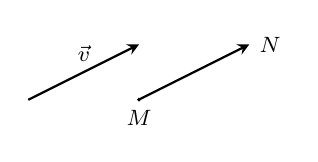
\begin{tikzpicture}[line join = round, line cap = round,>=stealth,thick,font=\footnotesize,scale=.7]
	\draw[->] (0,0)--(2,1);
	\draw[->] (2,0)--(4,1);
	\fill (2,0)node[below]{$M$} circle (1pt);
	\draw (1,0.5)node[above]{$\vec{v}$};
	\node at (4,1)[right]{$N$};
	\end{tikzpicture}
}
\textbf{b. Phép đối xứng qua mặt phẳng $(P)$ }
\immini{
	Là phép biến hình biến mỗi điểm thuộc $(P)$ thành chính nó, biến mỗi điểm $M$ không thuộc $(P)$ thành điểm $M’$ sao cho $(P)$ là mặt phẳng trung trực của $MM’$.\\
	Nếu phép đối xứng qua mặt phẳng $(P)$ biến hình $(H)$ thành chính nó thì $(P)$ được gọi là mặt phẳng đối xứng của $(H)$.
}{
	\begin{tikzpicture}[scale=0.8,>=stealth, font=\footnotesize, line join=round, line cap=round]
	\path
	(0,0) coordinate (A)
	(4,0) coordinate (B)
	(5,1.5) coordinate (C)
	($(A)-(B)+(C)$) coordinate (D)
	($(A)!0.5!(C)$) coordinate (I)
	(2.5,2.5) coordinate (M)
	($(M)!2!(I)$) coordinate (M')
	(intersection of I--M' and A--B) coordinate (K)
	(M)--(I)node[pos=0.4,sloped,rotate=-20]{$/$}
	(M')--(I)node[pos=0.4,sloped]{$/$}
	;
	\draw pic[draw,angle radius=4mm]{angle=B--A--D};
	\draw pic[draw=black,angle radius=0.2cm] {right angle = C--I--M}; %Lệnh đánh dấu góc vuông BAC
	\draw[dashed] (I)--(K);
	\draw (A)--(B)--(C)--(D)--cycle (M)--(I) (K)--(M')	;
	\foreach \i/\j in {I/150,M/30,M'/10} \fill[black] (\i)circle(1pt)($(\i)+(\j:3mm)$)node{\i};
\end{tikzpicture}
}

\textbf{c. Phép đối xứng qua tâm $O$ }
\immini{
Là phép biến hình biến điểm $O$ thành chính nó, biến mỗi điểm $M$ khác $O$ thành điểm $M’$ sao cho $O$ là trung điểm $MM’$.\\
Nếu phép đối xứng tâm $O$ biến hình $(H)$ thành chính nó thì $O$ được gọi là tâm đối xứng của $(H)$ 	
}{
	\begin{tikzpicture}[scale=0.8,>=stealth, font=\footnotesize, line join=round, line cap=round]
	\path
	(0,0) coordinate (M)
	(2,0.7) coordinate (O)
	($(M)!2!(O)$) coordinate (M')
	(M)--(O)node[pos=0.5,sloped]{$/$}
	(M')--(O)node[pos=0.5,sloped]{$/$}
	;
	\draw (M)--(M');
	\foreach \i/\j in {O/150,M/150,M'/10} \fill[black] (\i)circle(1pt)($(\i)+(\j:3mm)$)node{\i};
	\end{tikzpicture}
}

\textbf{d. Phép đối xứng qua đường thẳng $\Delta$ (phép đối xứng trục $\Delta$)}
\immini{
Là phép biến hình biến mọi điểm thuộc đường thẳng $\Delta$ thành chính nó, biến mỗi điểm $M$ không thuộc $\Delta$ thành điểm $M’$ sao cho $\Delta$ là đường trung trực của $MM’$.\\
Nếu phép đối xứng trục $\Delta$ biến hình $(H)$ thành chính nó thì $\Delta$ được gọi là trục đối xứng của $(H)$.
}{
		\begin{tikzpicture}[scale=0.8,>=stealth, font=\footnotesize, line join=round, line cap=round]
	\path
	(0,0) coordinate (M)
	(1.5,0.3) coordinate (I)
	($(M)!2!(I)$) coordinate (M')
	(M)--(I)node[pos=0.5,sloped]{$/$}
	(M')--(I)node[pos=0.5,sloped]{$/$}
	($(I)!1!-90:(M)!-.5!(I)$) coordinate (N)
	($(N)!1.7!(I)$) coordinate (N')
	;
	\draw pic[draw=black,angle radius=0.2cm] {right angle = M'--I--N'};
	\draw (M)--(M') (N')--(N)node[left] {$\Delta$};
	\foreach \i/\j in {I/150,M/150,M'/10} \fill[black] (\i)circle(1pt)($(\i)+(\j:3mm)$)node{\i};
	\end{tikzpicture}
}
\textbf{Nhận xét:}
\begin{itemize}
	\item Thực hiện liên tiếp các phép dời hình sẽ được một phép dời hình.
	\item Phép dời hình biến đa diện $(H)$ thành đa diện $(H’)$, biến đỉnh, cạnh, mặt của $(H)$ thành đỉnh, cạnh, mặt tương ứng của $(H’)$.
\end{itemize}
\textbf{2. Hai hình bằng nhau.}\\
Hai hình đa diện được gọi là bằng nhau nếu có một phép dời hình biến hình này thành hình kia.
\subsubsection{PHÂN CHIA VÀ LẮP GHÉP CÁC KHỐI ĐA DIỆN}
Nếu khối đa diện $(H)$ là hợp của hai khối đa diện $(H_1)$ và $(H_2)$ sao cho $(H_1)$ và $(H_2)$ không có chung điểm trong nào thì ta nói có thể phân chia được khối đa diện $(H)$ thành hai khối đa diện $(H_1)$ và $(H_2)$. Khi đó ta cũng nói có thể ghép hai khối đa diện $(H_1)$ và $(H_2)$ để được khối đa diện $(H)$.\\
\textbf{MỘT SỐ KẾT QUẢ QUAN TRỌNG.}
\begin{itemize}
	\item Kết quả 1: Một khối đa diện bất kì có ít nhất $4$ mặt.
	\item Kết quả 2: Mỗi hình đa diện có ít nhất $4$ đỉnh.
	\item Kết quả 3: Cho $(H)$ là đa diện mà các mặt của nó là những đa giác có $p$ cạnh. Nếu số mặt của $(H)$ là lẻ thì $p$ phải là số chẵn.\\
	\textbf{Chứng minh}
	Gọi $m$ là số các mặt của khối đa diện $(H)$. Vì mỗi mặt của $(H)$ có $p$ cạnh nên $m$ mặt sẽ có $pm$ cạnh. Nhưng do mỗi cạnh là cạnh chung của đúng hai đa giác nên số cạnh của $(H)$ bằng $c=\dfrac{pm}{2}$. Vì $m$ lẻ nên $p$ phải là số chẵn.
	\item Kết quả 4 (Suy ra từ chứng minh kết quả 3): Cho $(H)$ là đa diện có $m$ mặt, mà các mặt của nó là những đa giác có $p$ cạnh. Khi đó số cạnh của $(H)$ là $c=\dfrac{pm}{2}$.
	\item Kết quả 5: Mỗi khối đa diện có các mặt là các tam giác thì tổng số các mặt của nó phải là một số chẵn.\\
	Chứng minh: Gọi số cạnh và số mặt của khối đa diện lần lượt là $c$ và $m$.\\
	Vì mỗi mặt có ba cạnh và mỗi cạnh là cạnh chung của đúng hai mặt nên ta có số cạnh của đa diện là $c=\dfrac{3m}{2}$ (có thế áp dụng luôn kết quả 4 để suy ra $c=\dfrac{3m}{2}$).\\
	Suy ra $3m=2n\Rightarrow 3m$ là số chẵn $\Rightarrow m$ là số chẵn.\\
	Một số khối đa diện có đặc điểm như trên mà có số mặt bằng $4$, $6$, $8$, $10$:
	\begin{itemize}
		\item[+] Khối tứ diện $ABCD$ có $4$ mặt mà mỗi mặt là một tam giác.
		\item[+] Xét tam giác $BCD$ và hai điểm $A$, $E$ ở về hai phía của mặt phẳng $(BCD)$. Khi đó ta có khối lục diện $ABCDE$ có $6$ mặt là những tam giác.
		\item[+] Khối bát diện $ABCDEF$ có $8$ mặt là các tam giác.
		\item[+] Xét ngũ giác $ABCDE$ và hai điểm $M$, $N$ ở về hai phía của mặt phẳng chứa ngũ giác. Khi đó khối thập diện $MABCDEN$ có $10$ mặt là các tam giác.
		
	\end{itemize}
	\item Kết quả 6: Mỗi khối đa diện bất kì luôn có thể được phân chia được thành những khối tứ diện.
	\item Kết quả 7: Mỗi đỉnh của một hình đa diện là đỉnh chung của ít nhất $3$ cạnh.
	\item Kêt quả 8: Nếu khối đa diện có mỗi đỉnh là đỉnh chung của ba cạnh thì số đỉnh phải là số chẵn.\\
	Tông quát: Một đa diện mà mỗi đỉnh của nó đều là đỉnh chung của một số lẻ mặt thì tổng số đỉnh là một số chẵn.
	\item Kết quả 9: Mỗi hình đa diện có ít nhất $6$ cạnh.
	\item Kết quả 10: Không tồn tại hình đa diện có $7$ cạnh.
	\item Kết quà 11: Với mỗi số nguyên $k\geq 3$ luôn tồn tại hình đa diện có $2k$ cạnh.
	\item Kết quả 12: Với mỗi số nguyên $k\geq 4$ luôn tồn tại hình đa diện có $2k+1$ cạnh.
	\item Kết quả 13: Không tồn tại một hình đa diện có.\\
	+ Số mặt lớn hơn hoặc bằng số cạnh.\\
	+ Số đỉnh lớn hơn hoặc bằng số cạnh.
	\item Kết quả 14: Tồn tại khối đa diện có $2n$ mặt là những tam giác đều.\\
	Khối tứ diện đều có $4$ mặt là tam giác đều. Ghép hai khối tứ diện đều bằng nhau (một mặt của từ diện này ghép vào một mặt của tứ diện kia) ta được khối đa diện $(H_6)$ có $6$ mặt là tam giác đều. Ghép thêm vào $(H_6)$ một khối tứ diện đều nữa ta được khối đa diện $(H_8)$ có $8$ mặt là các tam giác đều. Bằng cách như vậy, ta được khốỉ đa diện có $2n$ mặt là các tam giác đều. \\
	\begin{center}
			\begin{tikzpicture}[scale=0.8,>=stealth, font=\footnotesize, line join=round, line cap=round]
	\path
	(0,0) coordinate (M)
	(3,1.5) coordinate (I)
	($(I)!1!20:(M)!-.5!(I)$) coordinate (N)
	($(I)!1!-25:(M)!-.5!(I)$) coordinate (N')
	($(I)!1!-60:(M)!-.2!(I)$) coordinate (A)
	;
	\draw[dashed] (N')--(I);
	\draw (M)--(I)--(N)--cycle
	      (M)--(N')--(A)--cycle (N')--(N) (A)--(I) ;
	\node at (N)[below=0.5]{$H_6$};
	\end{tikzpicture}
	\qquad
	\begin{tikzpicture}[scale=0.8,>=stealth, font=\footnotesize, line join=round, line cap=round]
	\path
	(0,0) coordinate (M)
	(3,1.5) coordinate (I)
	($(I)!1!20:(M)!-.5!(I)$) coordinate (N)
	($(I)!1!-22:(M)!-.5!(I)$) coordinate (N')
	($(I)!1!-60:(M)!-.2!(I)$) coordinate (A)
	($(I)!1!-27:(M)!-1.1!(I)$) coordinate (B)
	;
	\draw[dashed] (N')--(I) (B)--(N');
	\draw (M)--(I)--(N)--cycle
	(M)--(N')--(A)--cycle (N')--(N) (A)--(I) (M)--(B)--(A);
	\node at (N)[below=0.5]{$H_8$};
	\end{tikzpicture}
	\end{center}
\end{itemize}
\subsection{Phân loại và phương pháp giải bài tập}
\begin{dang}{Nhận diện, số đỉnh, số mặt, số cạnh của khối đa diện; phân chia lắp ghép khối đa diện}
\end{dang}
\subsubsection{Các ví dụ}
\begin{vd}%Ví dụ 1.%[2H1B1-2]
	Chứng minh rằng nếu khối đa diện có các mặt là những tam giác thì tổng các mặt của nó phải là một số chẵn. Hãy chỉ ra những khối đa diện như thế với số mặt bằng $4$, $6$, $8$, $10$
	\loigiai{
		Gọi số cạnh và số mặt của đa diện lần lượt là $c$ và $m$. Vì mỗi mặt có ba cạnh và mỗi cạnh là cạnh chung của đúng hai mặt nên ta có số cạnh của đa diện là $c=\dfrac{3m}{2}\Rightarrow 3m=2c\Rightarrow 3m$ chia hết cho $2$ mà $3$ không chia hết cho $2$ nên $m$ phải chia hết cho $2$, nghĩa là $m$ là số chẵn.\\
		* Khối đa diện $ABCD$ có $4$ mặt mà mỗi mặt là một tam giác.\\
		* Xét tam giác $BCD$ và hai điểm $A$, $E$ ở về hai phía của mặt phẳng $(BCD)$. Khi đó ta có khối lục diện $ABCDE$ có $6$ mặt là những tam giác.\\
		* Khối bát diện $ABCDEF$ có $8$ mặt là những tam giác.\\
		* Xét ngũ giác $ABCDE$ và hai điểm $M$, $N$ ở về hai phía của mặt phẳng chứa ngũ giác. Khi đó ta có khối thập diện $MABCDEN$ có $10$ mặt là những tam giác.}
%<MyLT>
\end{vd}
\begin{vd}%Ví dụ 2.%[2H1B1-2]
	Chứng minh rằng một đa diện mà mỗi đỉnh của nó đều là đỉnh chung của một số lẻ mặt thì tổng số các đỉnh của nó phải là một số chẵn
	\loigiai{
		Gọi $k$ là số đỉnh của đa diện và $C$ là số cạnh của đa diện.\\
		Ta có:\\
		-Tại đỉnh thứ $1$ có $(2n_1+1)$ mặt nên có $(2n_1+1)$ cạnh qua đỉnh thứ nhất.\\
		-Tại đỉnh thứ hai có $(2n_2+1)$ mặt nên có $(2n_2+1)$ cạnh qua đỉnh thứ hai.\\
		...\\
		-Tại đỉnh thứ $k$ có $(2n_k+1)$ mặt nên có $(2n_k+1)$ cạnh qua đỉnh thứ $k$.\\
		Mặt khác vì mỗi cạnh đi qua hai đỉnh nên ta có\\
		$2C=(2n_1+1)+(2n_2+1)+\cdots\cdot\cdot +(2n_k+1)=k+2\left(n_1+n_2+\cdots\cdot +n_k\right)\\\Rightarrow k=2\left[C-\left(n_1+n_2+\cdots\cdot +n_k\right)\right]$ \\
		$ \Rightarrow k $ là số chẵn (đpcm).}
%<MyLT>
\end{vd}
\begin{vd}%Ví dụ 3.%[2H1B1-2]
		Cho khối tứ diện đều $ABCD$. Chứng minh rằng:
	\begin{enumerate}
	\item Trọng tâm các mặt của khối đó là các đỉnh của một tứ diện đều.
	\item Các trung điểm các cạnh của khối đó là các đỉnh của một khối tám mặt đều	
	\end{enumerate}
	\loigiai{
	\begin{center}
		\begin{tikzpicture}[line join = round, line cap = round,>=stealth,thick,font=\footnotesize,scale=.7]
	\path
	(0:0) coordinate (B)
	(0:7) coordinate (D)
	($(B)!0.6!60:(D)$) coordinate (A)
	($(B)!0.8!-25:(D)$) coordinate (C)
	($(B)!0.5!(A)$) coordinate (P)
	($(B)!0.5!(C)$) coordinate (M)
	($(B)!0.5!(D)$) coordinate (S)
	($(D)!0.5!(A)$) coordinate (N)
	($(C)!0.5!(D)$) coordinate (Q)
	($(C)!0.5!(A)$) coordinate (R)
	($(M)!1/3!(A)$) coordinate (G)
	($(Q)!1/3!(A)$) coordinate (G')
	;
	\draw (A)--(B)--(C)--(D)--cycle (A)--(C) (P)--(M)--(R)--cycle (N)--(Q)--(R)--cycle (A)--(M) (A)--(Q)
	;
	\draw[dashed] (B)--(D) (M)--(Q)--(S)--cycle (P)--(S)--(N)--cycle (G)--(G')
	;
		\foreach \i/\j in {B/150,D/30,A/150,C/-30,P/150,M/-150,S/-90,N/30,Q/10,R/80} \fill[black] (\i)circle(1pt)($(\i)+(\j:3mm)$)node{\i};
		\fill (G) circle (1.0pt) node [left]{$G_1$};
		\fill (G') circle (1.0pt) node [right]{$G_2$};
	\end{tikzpicture}
	\end{center}
		1. Gọi $Q,M$ lần lượt là trung điểm của $CD,CB$; $G_1$, $G_2$, $G_3$, $G_4$ lần lượt là trọng tâm các mặt $(ABC)$, $(ACD)$, $(ABD)$ và $(BCD)$.\\
		Gọi $a$ là cạnh của tứ diện, ta có $G_1G_2=\dfrac{2}{3}MQ=\dfrac{2}{3}\dfrac{a}{2}=\dfrac{a}{3}$.\\
		Tương tự $G_1G_4=G_1G_3=G_2G_3 =G_2G_4=G_3G_4=\dfrac{a}{3}$ nên $G_1G_2G_3G_4$ là một tứ diện đều cạnh $\dfrac{a}{3}$.\\
		2. Gọi $N,P,R,S$ lần lượt là trung điểm các cạnh $AD$, $AB$, $AC$, $BD$.\\
		Theo tính chất đường trung bình, ta có:\\
		$QM=QN=QS=QR=PM=PN=PS=PR=\dfrac{a}{2}$.}
%<MyLT>
\end{vd}
\begin{vd}%Ví dụ 4.%[2H1B1-2]
	Với khối chóp tứ giác $S.ABCD$, xét hai khối chóp tam giác $S.ABC$ và $S.ACD$.\\
	Ta thấy rằng:\\
	Hai khối chóp $S.ABC$ và $S.ACD$ không có điểm trong chung (tức là không tồn tại điểm trong của khối chóp này là điểm trong của khối chóp kia và ngược lại).\\
	Hợp của hai khối chóp $S.ABC$ và $S.ACD$ chính là khối chóp $S.ABCD$. 
		\begin{center}
		\begin{tikzpicture}[line join = round, line cap = round,>=stealth,thick,font=\footnotesize,scale=.7]
		\path
		(0:0) coordinate (B)
		(-10:2) coordinate (C)
		($(B)!1.5!30:(C)$) coordinate (D)
		($(B)!1.5!80:(C)$) coordinate (S)
		($(B)!.5!150:(C)$) coordinate (A)
		;
		\draw (S)--(A)--(B)--cycle (B)--(C) (D)--cycle (S)--(C)--(D)--cycle
		;
		\draw[dashed] (A)--(D) (A)--(C)
		;
		\foreach \i/\j in {B/-90,D/30,A/150,C/-30,S/150} \fill[black] (\i)circle(1pt)($(\i)+(\j:3mm)$)node{\i};
		\end{tikzpicture}
	\end{center}
	
	Vậy khối chóp $S.ABCD$ được phân chia thành hai khối chóp $S.ABC$ và $S.ACD$ hay hai khối chóp $S.ABC$ và $S.ACD$ được ghép lại thành khối chóp $S.ABCD$.
%<MyLT>
\end{vd}
\begin{vd}%Ví dụ 5.%[2H1B1-2]
	Xét khối lập phương $ABCD.A’B’C’D’$. Mặt phẳng $BDD’B’$ cắt khối lập phương đó theo một thiết diện là hình chữ nhật $BDD’B’$. Thiết diện này chia các điểm còn lại của khối lập phương ra làm hai phần. Mỗi phần cùng với hình chữ nhật $BDD’B’$ tạo thành khối lăng trụ, như vậy có hai khối lăng trụ: $ABD\cdot A’B’D’$ và $BCD\cdot B’C’D’$.\\
	Khi đó ta nói mặt phẳng $(P)$ chia khối lập phương $ABCD.A’B’C’D’$ thành hai khối lăng trụ $ABD\cdot A’B’D’$ và $BCD\cdot B’C’D’$.\\
	Tương tự trên ta có thể chia tiếp khối trụ $ABD\cdot A’B’D’$ thành ba khối tứ diện: $ADBB’$, $ADB’D’$ và $AA’B’D’$. 
	\begin{center}
		\begin{tikzpicture}[>=stealth,line cap=round,line join=round]%[KV Thanh]
		\tikzset{c/.style={every coordinate/.try}}% Dùng để tịnh tiến các hình
		\coordinate (a) at (0,0);
		\coordinate (a') at (0,-2);
		\coordinate (b) at (0.5,1);
		\coordinate (d) at (2,0);
		\coordinate (c) at ($(b)+(d)-(a)$);
		\coordinate (b') at ($(b)+(a')-(a)$);
		\coordinate (d') at ($(a')+(d)-(a)$);
		\coordinate (c') at ($(c)+(d')-(d)$);	
		\coordinate (o) at ($(a)+(2.7,-0.1)$); tọa độ gốc 2 mũi tên thứ 1
		\def\x{4}; % Xác định tọa độ của véc tơ tịnh tiến các hình (x,y)
		\def\y{2};
		\def\z{-2};
		% Vẽ hình 1
		\draw[dashed, fill=black!20] (b)--(d)--(d')--(b')--cycle;
		\draw [dashed] (a')--(b')--(c') node at ($(b')+(-.2,0)$) {$B'$};
		\draw (a) node[above left]{$A$}--(b) node[above]{$B$}--(c) node[above]{$C$}--(d) node[above]{$D$}--cycle;
		\draw (a)--(a') node[below left]{$A'$}--(d') node[below]{$D'$}--(d);
		\draw (c) --(c') node[right]{$C'$}--(d');
		\draw (b) --(d)--(d');
		% Vẽ hình 2 tịnh tiến từ một phần của hình 1 theo véc tơ (x,y)
		\begin{scope}[every coordinate/.style={shift={(\x,\y)}}]
		\draw[dashed] ([c]b')--([c]c');
		\draw ([c]b) node[above left]{$B$} --([c]c) node[above right]{$C$}--([c]d) node[below left]{$D$}--cycle;
		\draw ([c]b)--([c]b') node[left]{$B'$}--([c]d') node[below]{$D'$}--([c]c') node[right]{$C'$}--([c]c);
		\draw ([c]d)--([c]d');	
		\end{scope}
		%Vẽ hình 3
		\begin{scope}[every coordinate/.style={shift={(\x,\z)}}]
		\draw [dashed] ([c]a')--([c]b');
		\draw[dashed, fill=gray!20] ([c]a)--([c]b')node at ($([c]b')+(-.3,-.1)$) {$B'$}--([c]d')--cycle;
		\draw [dashed] ([c]b)--([c]b')--([c]d);
		\draw ([c]a) node[above left]{$A$}--([c]b) node[above]{$B$}--([c]d) node[above right]{$D$}--cycle;
		\draw ([c]a)--([c]a') node[below]{$A'$}--([c]d') node[below]{$D'$}--([c]d);
		\draw ([c]a)--([c]d');
		\end{scope}
		%Hình 4
		\begin{scope}[every coordinate/.style={shift={(\x+\x,\y+\z)}}]
		%\draw[dashed, fill=gray!20] ([c]a)--([c]b')--([c]d)--cycle;
		\draw[draw=none, fill=gray!20] ([c]a)--([c]b')--([c]d)--cycle;
		\draw [dashed] ([c]b)--([c]b')--([c]d);
		\draw ([c]a) node[left]{$A$}--([c]b) node[above]{$B$}--([c]d) node[above right]{$D$}--cycle;
		\draw ([c]a)--([c]d') node[below]{$D'$}--([c]d);
		\draw ([c]a)--([c]b') node[below left]{$B'$}--([c]d');
		\end{scope}
		%Vẽ hình 5
		\begin{scope}[every coordinate/.style={shift={(\x+\x,\z+\z)}}]
		\draw [dashed] ([c]a')--([c]b')--([c]d');
		\draw [dashed] ([c]a)--([c]b');
		\draw ([c]a) node[above]{$A$}--([c]a') node[below]{$A'$}--([c]d') node[below right]{$D'$}--cycle;
		\end{scope}
		%Vẽ hình 6
		\begin{scope}[every coordinate/.style={shift={(\x+\x+\x,\y+\y+\z)}}]
		\draw [dashed] ([c]b)--([c]b');
		\draw ([c]a)--([c]b') node[below]{$B'$}--([c]d);
		\draw ([c]a) node[left]{$A$}--([c]b) node[above]{$B$}--([c]d) node[right]{$D$}--cycle;
		\end{scope}
		%Vẽ hình 7
		\begin{scope}[every coordinate/.style={shift={(\x+\x+\x,\y+\z+\z)}}]
		\draw [dashed] ([c]d)--([c]b');
		\draw ([c]a)--([c]b') node[below left]{$B'$}--([c]d');
		\draw ([c]a) node[above]{$A$}--([c]d) node[above right]{$D$}--([c]d') node[below right]{$D'$}--cycle;
		\end{scope}	
		%Vẽ các mũi tên
		\coordinate (i) at ($(o)+(1,0.8)$);
		\coordinate (j) at ($(o)+(1,-0.8)$);
		\draw[black,->] (o) -- (i);
		\draw[black,->] (o) -- (j);
		\begin{scope}[every coordinate/.style={shift={(\x,\z-0.5)}}]
		\draw[black,->] ([c]o) -- ([c]i);
		\draw[black,->] ([c]o) -- ([c]j);
		\end{scope}
		\begin{scope}[every coordinate/.style={shift={(\x+\x,\z-0.5+\y)}}]
		\draw[black,->] ([c]o) -- ([c]i);
		\draw[black,->] ([c]o) -- ([c]j);
		\end{scope}	
		\end{tikzpicture}\newline
	\end{center}
%<MyLT>
\end{vd}
\paragraph{Câu hỏi trắc nghiệm}
\begin{ex}%[2H1Y1-1] %Câu 1.
	Mỗi hình sau gồm một hữu hạn đa giác phẳng (kể cả các điểm trong của nó). 
	\begin{center}
		\begin{tabular}{c c c c}
			\begin{tikzpicture}[line join=round,line width=.6pt,scale=.7]
			\path
			(0,0) coordinate (A) ++(45:1.6) coordinate (B) ++(0:2.8) coordinate (C) ++(-135:1.6) coordinate (D)
			(70:2.3) coordinate (A') ++(45:.8) coordinate (B') ++(0:1.4) coordinate (C') ++(-135:.8) coordinate (D')
			($(A')+(0,.8)$) coordinate (A'') ++(45:.8) coordinate (B'') ++(0:1.4) coordinate (C'') ++(-135:.8) coordinate (D'');
			\draw (A)--(D)--(C)--(C')--(C'')--(B'')--(A'')--(A')--cycle 
			(A')--(D')--(C') (A'')--(D'')--(C'') (D)--(D')--(D'');
			\draw[dashed] (A)--(B)--(C) (A')--(B')--(C') (B)--(B')--(B'');
			\end{tikzpicture}
			& 
			\begin{tikzpicture}[line join=round,line width=.6pt,scale=.7]
			\path
			(0,0) coordinate (A) ++(120:1.4) coordinate (B) ++(0:2.4) coordinate (C) ++(-60:1.4) coordinate (D)
			($(A)+(0,1.6)$) coordinate (A') ++(120:1.4) coordinate (B') ++(0:2.4) coordinate (C') ++(-60:1.4) coordinate (D')
			($(B')+(60:1.2)$) coordinate (A'') ++(0:2.4) coordinate (B'');
			\draw (A)--(A')--(D')--(D)--(A)--(B)--(B')-- (A') (D')--(C')--(B')--(A'')--(B'')--(C');
			\draw[dashed] (B)--(C)--(D) (C)--(C');
			\end{tikzpicture}
			&
			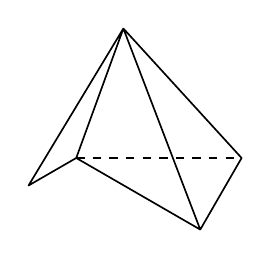
\begin{tikzpicture}[line join=round,line width=.6pt,scale=.7]
			\path
			(0,0) coordinate (A) ++(0:3) coordinate (B) ++(-120:1.5) coordinate (C) 
			(-150:1) coordinate (D) (70:2.5) coordinate (E);
			\draw (A)--(D)--(E)--(A)--(C)--(B)--(E)--(C);
			\draw[dashed] (A)--(B);
			\end{tikzpicture}
			&
			\begin{tikzpicture}[line join=round,line width=.6pt,scale=.7]
			\path
			(0,0) coordinate (A) ++(120:1.4) coordinate (B) ++(0:2.4) coordinate (C) ++(-60:1.4) coordinate (D)
			($(A)+(0,1.6)$) coordinate (A') ++(120:1.4) coordinate (B') ++(0:2.4) coordinate (C') ++(-60:1.4) coordinate (D')
			($(B')!.25!(C')$) coordinate (M) ($(A')!.55!(D')$) coordinate (N)
			($(M)+(105:1)$) coordinate (A'') ++(.5,0) coordinate (B'') ($(N)-(M)+(B'')$) coordinate (C'')
			++(-.5,0) coordinate (D'');
			\coordinate (P) at (intersection of B'--C' and B''--C'');
			\draw (A)--(A')--(D')--(D)--(A)--(B)--(B')-- (A') (D')--(C') 
			(A'')--(B'')--(C'')--(D'')--(A'')--(M)--(N)--(D'')  (N)--(C'') (B')--(M) (P)--(C');
			\draw[dashed] (B)--(C)--(D) (C)--(C') (B'')--(M)--(P);
			\end{tikzpicture}\\
			Hình (a)&Hình (b)&Hình (c)&Hình (d) \vphantom{$ \dfrac{text}{den} $}
		\end{tabular} 
	\end{center}
	Hnh đa diện là
	\choice
	{\True hình (a)}
	{hình (b)}
	{hình (c)}
	{hình (d)}
	\loigiai{}
\end{ex}
\begin{ex}%[2H1Y1-1] %Câu 2.
	Mỗi hình sau gồm một hữu hạn đa giác phẳng (kể cả các điểm trong của nó). 
	\begin{center}
		\begin{tabular}{c c c c}
			\begin{tikzpicture}[line join=round,line width=.6pt,scale=.7]
			\path
			(0,0) coordinate (A) ++(45:1.6) coordinate (B) ++(0:2.8) coordinate (C) ++(-135:1.6) coordinate (D)
			(70:2.3) coordinate (A') ++(45:.8) coordinate (B') ++(0:1.4) coordinate (C') ++(-135:.8) coordinate (D')
			($(A')+(0,.8)$) coordinate (A'') ++(45:.8) coordinate (B'') ++(0:1.4) coordinate (C'') ++(-135:.8) coordinate (D'');
			\draw (A)--(D)--(C)--(C')--(C'')--(B'')--(A'')--(A')--cycle 
			(A')--(D')--(C') (A'')--(D'')--(C'') (D)--(D')--(D'');
			\draw[dashed] (A)--(B)--(C) (A')--(B')--(C') (B)--(B')--(B'');
			\end{tikzpicture}
			&
			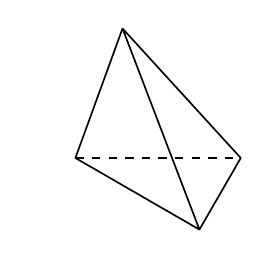
\begin{tikzpicture}[line join=round,line width=.6pt,scale=.7]
			\path
			(0,0) coordinate (A) ++(0:3) coordinate (B) ++(-120:1.5) coordinate (C) 
			(-150:1) coordinate (D) (70:2.5) coordinate (E);
			\draw (E)--(A)--(C)--(B)--(E)--(C)
			;
			\draw[dashed] (A)--(B);
			\end{tikzpicture}
			& 
			\begin{tikzpicture}[line join=round,line width=.6pt,scale=.7]
			\path
			(0,0) coordinate (A) ++(120:1.4) coordinate (B) ++(0:2.4) coordinate (C) ++(-60:1.4) coordinate (D)
			($(A)+(0,1.6)$) coordinate (A') ++(120:1.4) coordinate (B') ++(0:2.4) coordinate (C') ++(-60:1.4) coordinate (D')
			($(B')+(60:1.2)$) coordinate (A'') ++(0:2.4) coordinate (B'');
			\draw (A)--(A')--(D')--(D)--(A)--(B)--(B')-- (A') (D')--(C')--(B')
			;
			\draw[dashed] (B)--(C)--(D) (C)--(C');
			\end{tikzpicture}
			&
			\begin{tikzpicture}[line join=round,line width=.6pt,scale=.7]
			\path
			(0,0) coordinate (A) ++(120:1.4) coordinate (B) ++(0:2.4) coordinate (C) ++(-60:1.4) coordinate (D)
			($(A)+(0,1.6)$) coordinate (A') ++(120:1.4) coordinate (B') ++(0:2.4) coordinate (C') ++(-60:1.4) coordinate (D')
			($(B')!.25!(C')$) coordinate (M) ($(A')!.55!(D')$) coordinate (N)
			($(M)+(105:1)$) coordinate (A'') ++(.5,0) coordinate (B'') ($(N)-(M)+(B'')$) coordinate (C'')
			++(-.5,0) coordinate (D'');
			\coordinate (P) at (intersection of B'--C' and A''--D'');
			\draw (A)--(A')--(D')--(D)--(A)--(B)--(B')-- (A') (D')--(C') 
			(A'')--(D'')--(A'')--(M)--(N)--(D'')   (B')--(M) (P)--(C')
			;
			\draw[dashed] (B)--(C)--(D) (C)--(C') (M)--(P) ;
			\end{tikzpicture}\\
			Hình (a)&Hình (b)&Hình (c)&Hình (d) \vphantom{$ \dfrac{text}{den} $}
		\end{tabular} 
	\end{center}
	Hình \textbf{không} phải đa diện là
	\choice
	{hình (a)}
	{hình (b)}
	{hình (c)}
	{\True hình (d)}
	\loigiai{.}
\end{ex}
\begin{ex}%[2H1Y1-1] %Câu 3.
	Hình nào trong các hình sau \textbf{không} phải là hình đa diện?
	\choice
	{Hình chóp}
	{\True Hình vuông}
	{Hình lập phương}
	{Hình lăng trụ}
	\loigiai{.}
\end{ex}
\begin{ex}%[2H1Y2-1]%Câu 4.
	Cho các hình khối sau: 
\begin{center}
	\begin{tikzpicture}[scale=.4, font=\footnotesize, line join=round, line cap=round, >=stealth]
\def \c{5}	\def \b{4}	
\def \d{2.5}	\def \goc{45}
\def \h{3.5}	
\path
(0,0) coordinate (A)
(\b,0) coordinate (B)
(\goc:\d) coordinate (D)
($(B)+(D)-(A)$) coordinate (C)
($(A)!.5!(C)$) coordinate (O)
($(O)+(0,\h)$) coordinate (S)
($(S)!.4!(A)$) coordinate (A1)
($(S)!.4!(B)$) coordinate (B1)
($(S)!.4!(C)$) coordinate (C1)
($(S)!.4!(D)$) coordinate (D1)
;
\draw [dashed] (A)--(D)--(C) (D)--(D1);
\draw (A)--(B)--(C)--(C1)--(B1)--(A1)--(D1)--(C1) (A)--(A1) (B)--(B1);
\path (\b/2,-1) node {$(a)$};
\end{tikzpicture}
\quad \quad
\begin{tikzpicture}[scale=.4, font=\footnotesize, line join=round, line cap=round, >=stealth]
\def \c{5}	\def \b{4}	
\def \d{2}	\def \goc{120}
\def \h{2}	\def \k{.7}
\path
(0,0) coordinate (A)
(\b,0) coordinate (B)
(\goc:\d) coordinate (D)
($(B)+(D)-(A)$) coordinate (C)
($(O)+(0,\h)$) coordinate (S)
($(A)+(0,\h)$) coordinate (A1)
($(B)+(0,\h)$) coordinate (B1)
($(C)+(0,\h)$) coordinate (C1)
($(D)+(0,\h)$) coordinate (D1)
($(D1)!.25!(C1)$) coordinate (H)
($(A1)!.45!(B1)$) coordinate (K)
($(H)+(-.4,\k)$) coordinate (H1)
($(H)+(.4,\k)$) coordinate (H2)
($(K)+(-.4,\k)$) coordinate (K1)
($(K)+(.4,\k)$) coordinate (K2)
;
\draw [dashed] (D)--(C)--(B) (C)--(C1) (H)--(H2);
\draw (D1)--(C1)--(B1)--(A1)--(D1)--(D)--(A)--(B) (A)--(A1) (B)--(B1) (H)--(K) (H)--(H1)--(H2)--(K2)--(K1)--(H1) (K1)--(K)--(K2);
\path (\b/2,-1) node {$(b)$};
\end{tikzpicture}
\quad \quad
\begin{tikzpicture}[scale=.4, font=\footnotesize, line join=round, line cap=round, >=stealth]
\def \c{5}	\def \b{4}	
\def \d{2}	\def \goc{120}
\def \h{2}	\def \k{.7}
\path
(0,0) coordinate (A)
(\b,0) coordinate (B)
(\goc:\d) coordinate (D)
($(B)+(D)-(A)$) coordinate (C)
($(O)+(0,\h)$) coordinate (S)
($(A)+(0,\h)$) coordinate (A1)
($(B)+(0,\h)$) coordinate (B1)
($(C)+(0,\h)$) coordinate (C1)
($(D)+(0,\h)$) coordinate (D1)
;
\draw [dashed] (D)--(C)--(B) (C)--(C1);
\draw (D1)--(C1)--(B1)--(A1)--(D1)--(D)--(A)--(B) (A)--(A1) (B)--(B1);
\path (\b/2,-1) node {$(c)$};
\end{tikzpicture}
\quad \quad
\begin{tikzpicture}[scale=.4, font=\footnotesize, line join=round, line cap=round, >=stealth]
\def \c{5}	\def \b{4}	
\def \d{2}	\def \goc{120}
\def \h{2}	\def \k{.7}
\path
(0,0) coordinate (A)
(\b,0) coordinate (B)
(\goc:\d) coordinate (D)
($(B)+(D)-(A)$) coordinate (C)
($(O)+(0,\h)$) coordinate (S)
($(A)+(0,\h)$) coordinate (A1)
($(B)+(0,\h)$) coordinate (B1)
($(C)+(0,\h)$) coordinate (C1)
($(D)+(0,\h)$) coordinate (D1)
($(D1)!.2!(C1)$)+(0,\k) coordinate (H)
($(A1)!.2!(B1)$)+(0,\k) coordinate (K)
;
\draw [dashed] (D)--(C)--(B) (C)--(C1)--(D1);
\draw (C1)--(B1)--(A1)--(D1)--(D)--(A)--(B) (A)--(A1) (B)--(B1) (H)--(K) (A1)--(K)--(B1) (D1)--(H)--(C1);
\path (\b/2,-1) node {$(d)$};
\end{tikzpicture}
\end{center}
	Mỗi hình trên gồm một số hữu hạn đa giác phẳng (kể cả các điểm trong của nó), hình không phải đa diện lồi là
	\choice
	{hình (a)}
	{\True hình (b)}
	{hình (c)}
	{hình (d)}
	\loigiai{
		Nhận thấy tọa độ điểm $M$ thỏa mãn phương trình đường thẳng $d$.}
\end{ex}
%\begin{ex}%[2H1Y2-1]%Câu 5.
%	Cho các hình khối sau: 
%\begin{center}
%	\begin{tikzpicture}[line cap=round,line join=round,>=stealth,x=1.0cm,y=1.0cm,scale=.7]
%\draw(0,0) -- (4,0)--(6,1)--(5,4)--(3,4)--(2,3)--(0,0);
%\draw[dashed](0,0) -- (2,1)--(3,4);
%\draw[dashed](2,1) -- (6,1);
%\draw(5,4) -- (4,3)--(2,3);
%\draw(4,0) -- (4,3); 

%\draw(9,0) -- (8,1)--(8,4)--(9,3)--(9,0)--(13,0)--(13,3)--(12,4)--(10.61,4)--(11.26,3.56)--(10.81,3)--(10.44,3.56)--(11.26,3.56);
%\draw(9,3) -- (13,3);
%\draw(8,4) -- (9.33,4)--(10.81,3);
%\draw(10.44,3.56) -- (8.96,4.56)--(9.33,4);
%\draw(8.96,4.56) -- (9.78,4.56)--(11.26,3.56);
%\draw[dashed](9.33,4) -- (10.61,4);
%\draw[dashed](8,1) -- (12,1)--(12,4);
%\draw[dashed](12,1) -- (13,0);

%\draw(15,0) -- (17,0)--(19,2)--(19,2.78)--(17,0.78)--(17,0);
%\draw(17,0.78) -- (16,0.78)--(18,2.78)--(19,2.78);

%\draw(15,0) -- (15,2)--(16,2)--(16,0.78)--(18,2.78)--(18,4)--(16,2)--(15,2);
%\draw(15,2) -- (17,4)--(18,4);
%\draw[dashed](15,0) -- (17,2)--(17,4);
%\draw[dashed](17,2) -- (19,2);

%\draw(21,0) -- (24,0);
%\draw[dashed](23,1)--(20,1);
%\draw(20,3)--(20.7,3.7)--(21.7,2.7)--(21,2);
%\draw(21,2) -- (21,0);
%\draw(21,0) -- (20,1);
%\draw(21,2) -- (20,3);
%\draw(21,2) -- (24,2);
%\draw(24,0) -- (24,2)--(21.7,2.7);
%\draw(20,1) -- (20,3);
%\draw[dashed](24,0) -- (23,1);
%\draw(24,2) -- (23,3)--(20.7,3.71);
%\draw[dashed](20,3) -- (23,3);
%\draw[dashed](23,1) -- (23,3);
%\tkzLabelPoint[below](2.87,-1.17){a)};
%\tkzLabelPoint[below](10.72,-1.17){b)};
%\tkzLabelPoint[below](17.26,-1.17){c)};
%\tkzLabelPoint[below](22.14,-1.17){d)};
%\end{tikzpicture} 
%\end{center}
%	Mỗi hình trên gồm một số hữu hạn đa giác phẳng (kể cả các điểm trong của nó), số đa diện lồi là
%	\choice
%	{$1$}
%	{\True $2$}
%	{$3$}
%	{$4$}
%	\loigiai{.}
%\end{ex}
\begin{ex}%[2H1Y1-2]%Câu 6.
	\immini{
		Hình đa diện trong hình vẽ sau có bao nhiêu mặt?
		\choice
		{$8$}
		{\True $10$}
		{$11$}
		{$12$}
	}{
		
			\begin{tikzpicture}[line cap=round,line join=round,>=stealth,x=1.0cm,y=1.0cm,scale=.7]
			\def\d{4}
			\def\c{3}
			\path 
			(0,0) coordinate (A)
			(\d-2,0) coordinate (B)
			(-2,-2) coordinate (C)
			(2,-2) coordinate (D)
			(4,-1) coordinate (E)
			($(A)+(1,\c)$) coordinate (S)
			($(A)+(1.5,-\c-1)$) coordinate (S')
			;
			\draw[-] (C)--(D)--(E)
			;
			\foreach \i in {C,D,E} \draw[-] (S)--(\i) (S')--(\i);
			\draw[dashed] (S')--(A)--(B)--cycle
			(A)--(C) (A)--(S)--(B)--(E) ;
			%\foreach \i/\j in {A/150,B/30,C/-70,D/-120,E/50,S/30} \fill[black] (\i)circle(1pt) ($(\i)+(\j:3mm)$)node{\i};
			\end{tikzpicture}
	} 
	\loigiai{.}
\end{ex}
\begin{ex}%[2H1Y1-2]%Câu 7.
	\immini{
		Hình đa diện trong hình vẽ sau có bao nhiêu mặt?
		\choice
		{$11$}
		{\True $12$}
		{$13$}
		{$14$}
	}{
	\begin{tikzpicture}[line cap=round,line join=round,>=stealth,x=1.0cm,y=1.0cm,scale=.7]
	\tkzDefPoints{0/1/A,1.5/0.22/B,4.44/0.5/C,5.84/1.6/D,3.26/2.32/E,0.04/2.4/F,1.94/1.52/G,4.3/1.66/H,5.92/3.18/I,3.4/3.5/K,1.86/4.82/L,2.74/4.44/M,3.56/4.64/N,3.66/5.18/O,3.04/5.34/P}'
	\tkzDrawSegments(A,B B,C C,D D,I I,H H,G G,F A,F B,G C,H D,I L,M M,N N,O O,P P,L F,L G,M H,N I,O);
	\tkzDrawSegments[dashed](A,E E,D F,K K,I K,P E,K);
	\end{tikzpicture} 
	} 
	\loigiai{.}
\end{ex}
\begin{ex}%[2H1Y1-2]%Câu 8.
\immini{
		Hình đa diện sau có bao nhiêu cạnh?
	\choice
	{$21$}
	{$22$}
	{\True $23$}
	{$24$}
}{
	\begin{tikzpicture}[line cap=round,line join=round,>=stealth,x=1.0cm,y=1.0cm,scale=.8]
	\tkzDefPoints{2/0/A,0/1/B,0/2.5/C,0.52/3.76/D,2.18/3.2/E,4.66/4.48/F,4.64/3.38/G,6.2/2.76/H,5/1/I,4.22/1.9/K,2.38/1.76/L,1.74/0.94/M,3.46/1.48/N,3.36/2.42/O}
	
	\tkzDrawSegments(A,B B,C C,D D,F F,G G,H G,O O,N N,I N,A A,I I,N I,H F,H C,O);
	\tkzDrawSegments[dashed](B,M M,A M,L L,K K,H L,E E,D E,F K,I);
	
	\end{tikzpicture} 
}
	\loigiai{.}
\end{ex}
\begin{ex}%[2H1Y1-2]%Câu 9.
	Cho một hình đa diện. Trong các khẳng định sau, khẳng định nào \textbf{sai}?
	\choice
	{Mỗi đỉnh là đỉnh chung của ít nhất ba cạnh}
	{Mỗi mặt có ít nhất ba cạnh}
	{\True Mỗi cạnh là cạnh chung của ít nhất ba mặt}
	{Mỗi đỉnh là đỉnh chung của ít nhất ba mặt}
	\loigiai{.}
\end{ex}
\begin{ex}%[2H1Y1-2]%Câu 10.
	Phát biểu nào sau đây là đúng?
	\choice
	{\True Khối đa diện $S.A_1A_2\cdots A_n$ có đúng $n+1$ mặt}
	{Khối đa diện $S.A_1A_2\cdots A_n$ có đúng $n+1$ cạnh}
	{Khối đa diện $S.A_1A_2\cdots A_n$ có đúng $n$ đỉnh}
	{Khối đa diện $S.A_1A_2\cdots A_n$ có đúng $n$ cạnh}
	\loigiai{.}
\end{ex}
\begin{ex}%[2H1Y1-2]%Câu 11.
	Phát biểu nào sau đây là đúng?
	\choice
	{Hình tứ diện đều có $6$ đỉnh, $6$ cạnh, $4$ mặt}
	{Hình tứ diện đều có $4$ đỉnh, $4$ cạnh, $4$ mặt}
	{Hình tứ diện đều có $6$ đỉnh, $4$ cạnh, $4$ mặt}
	{\True Hình tứ diện đều có $4$ đỉnh, $6$ cạnh, $4$ mặt}
	\loigiai{.}
\end{ex}
\begin{ex}%[2H1Y1-2]%Câu 12.
	Phát biểu nào sau đây là đúng?
	\choice
	{\True Hình lập phương có $8$ đỉnh, $12$ cạnh, $6$ mặt}
	{Hình lập phương có $6$ đỉnh, $12$ cạnh, $8$ mặt}
	{Hình lập phương có $12$ đỉnh, $8$ cạnh, $6$ mặt}
	{Hình lập phương có $8$ đỉnh, $6$ cạnh, $12$ mặt}
	\loigiai{.}
\end{ex}
\begin{ex}%[2H1Y1-2]%Câu 13.
	Phát biểu nào sau đây là đúng?
	\choice
	{Hình bát diện đều có $8$ đỉnh, $12$ cạnh, $6$ mặt}
	{\True Hình bát diện đều có $6$ đỉnh, $12$ cạnh, $8$ mặt}
	{Hình bát diện đều có $12$ đỉnh, $8$ cạnh, $6$ mặt}
	{Hình bát diện đều có $8$ đỉnh, $6$ cạnh, $12$ mặt}
	\loigiai{.}
\end{ex}
\begin{ex}%[2H1Y1-2]%Câu 14.
	Trong các mệnh đề sau, mệnh đề nào đúng?
	\choice
	{\True Mỗi hình đa diện có ít nhất bốn đỉnh}
	{Mỗi hình đa diện có ít nhất ba cạnh}
	{Số đỉnh của một hình đa diện lớn hơn hoặc bằng số cạnh của nó}
	{Số mặt cảu một hình đa diện lớn hơn hoặc bằng số cạnh của nó}
	\loigiai{.}
\end{ex}

\begin{ex}%[BCO Tuan, dự án DCHT]%[2H1B1-2]%Câu 15.
	Cho khối chóp có đáy là đa giác lồi có $7$ cạnh. Trong các mệnh đề sau mệnh đề nào đúng?
	\choice
	{Số đỉnh của khối chóp bằng $15$}
	{\True Số mặt của khối chóp bằng số đỉnh của nó}
	{Số mặt của khối chóp bằng $14$}
	{Số cạnh của khối chóp bằng}
	\loigiai{Số mặt của khối chóp bằng số đỉnh của nó.}
\end{ex}
\begin{ex}%[BCO Tuan, dự án DCHT]%[2H1B1-2]%Câu 16.
	Khối đa diện có các mặt đều là tam giác. Trong các mệnh đề sau, mệnh đề nào đúng?
	\choice
	{Số mặt và số đỉnh của nó bằng nhau}
	{Số mặt và số cạnh của nó bằng nhau}
	{\True Số mặt của nó là số chẵn}
	{Số mặt của nó là số lẻ}
	\loigiai{Số mặt của khối đa diện có các mặt đều là tam giác là số chẵn.}
\end{ex}
\begin{ex}%[BCO Tuan, dự án DCHT]%[2H1B1-2]%Câu 17.
	Trong các mệnh đề sau, mệnh đề nào sai?
	\choice
	{\True Tồn tại hình đa diện có số cạnh bằng $7$}
	{Tồn tại một hình đa diện có số cạnh nhỏ hơn $7$}
	{Số cạnh đa diện luôn luôn lớn hơn hoặc bằng $6$}
	{Tồn tại hình đa diện có số cạnh lớn hơn $7$}
	\loigiai{
		Không tồn tại hình đa diện có số cạnh bằng $7$.	
	}
\end{ex}
\begin{ex}%[BCO Tuan, dự án DCHT]%[2H1B1-2]%Câu 18.
	Trong các mệnh đề sau, mệnh đề nào đúng?
	\choice
	{Trong một hình đa diện tổng số mặt và số cạnh nhỏ hơn số đỉnh}
	{\True Trong một hình đa diện tổng của số mặt và số đỉnh lớn hơn số cạnh}
	{Trong một hình đa diện tổng của số cạnh và số đỉnh nhỏ hơn số mặt}
	{Tồn tại một hình đa diện có tổng của số mặt và số đỉnh nhỏ hơn số cạnh}
	\loigiai{
		Theo công thức Ơle: $d+m-c=2$. Nên trong một hình đa diện tổng của số mặt và số đỉnh lớn hơn số cạnh.}
\end{ex}
\begin{ex}%[BCO Tuan, dự án DCHT]%[2H1B1-2]%Câu 19.
	Một hình chóp có $46$ cạnh có bao nhiêu mặt?
	\choice
	{\True $24$}
	{$46$}
	{$69$}
	{$25$}
	\loigiai{
		Giả sử đa giác đáy có $n$ cạnh. Suy ra đa diện có $2n$ cạnh. Suy ra $2n=46\Leftrightarrow n=23$.\\
		Suy ra có $23$ mặt bên và $1$ mặt đáy. Do đó có tổng cộng là $24$ mặt.}
\end{ex}
\begin{ex}%[BCO Tuan, dự án DCHT]%[2H1B1-2]%Câu 20.
	Một hình đa diện có các mặt là những tam giác thì số mặt $M$ và số cạnh $C$ của đa diện đó thoả mãn
	\choice
	{$3C=2M$}
	{$C=M+2$}
	{$M\geq C$}
	{\True $3M=2C$}
	\loigiai{
		Đáp án là $3M=2C$.	
	}
\end{ex}
\begin{ex}%[BCO Tuan, dự án DCHT]%[2H1B1-3]%Câu 21.
	Cho khối lăng trụ tam giác đều $ABC.A’B’C’$. Về phía ngoài khối lăng trụ này ta ghép thêm một khối lăng trụ tam giác đều bằng với khối lăng trụ đã cho, sao cho hai khối lăng trụ có chung một mặt bên. Hỏi khối đa diện mới lập thành có mấy cạnh?
	\choice
	{$9$}
	{\True $12$}
	{$15$}
	{$18$}
	\loigiai{
		Khối lăng trụ lập thành là một khối lăng trụ đứng tứ giác nên có $12$ cạnh
		\begin{center}
			\begin{tikzpicture}[>=stealth,line cap=round,line join=round]%[KV Thanh]
			\tikzset{c/.style={every coordinate/.try}}% Dùng để tịnh tiến các hình
			\coordinate (a) at (0,0);
			\coordinate (a') at (0,-2);
			\coordinate (b) at (0.5,1);
			\coordinate (d) at (2,0);
			\coordinate (c) at ($(b)+(d)-(a)$);
			\coordinate (b') at ($(b)+(a')-(a)$);
			\coordinate (d') at ($(a')+(d)-(a)$);
			\coordinate (c') at ($(c)+(d')-(d)$);	
			\coordinate (o) at ($(a)+(2.7,-0.1)$); tọa độ gốc 2 mũi tên thứ 1
			\def\x{4}; % Xác định tọa độ của véc tơ tịnh tiến các hình (x,y)
			\def\y{2};
			\def\z{-2};
			% Vẽ hình 1
			\draw[dashed, fill=black!20] (b)--(d)--(d')--(b')--cycle;
			\draw [dashed] (a')--(b')--(c');
			\draw (a) --(b) --(c) --(d) --cycle;
			\draw (a)--(a') --(d') --(d);
			\draw (c) --(c')--(d');
			\draw (b) --(d)--(d');
			% Vẽ hình 2 tịnh tiến từ một phần của hình 1 theo véc tơ (x,y)
			\begin{scope}[every coordinate/.style={shift={(\x,\y)}}]
			\draw[dashed] ([c]b')--([c]c');
			\draw ([c]b) node[above left]{$B$} --([c]c) node[above right]{$C$}--([c]d) node[below left]{$A$}--cycle;
			\draw ([c]b)--([c]b') node[left]{$B'$}--([c]d') node[below]{$A'$}--([c]c') node[right]{$C'$}--([c]c);
			\draw ([c]d)--([c]d');	
			\end{scope}
			%Vẽ hình 3
			\begin{scope}[every coordinate/.style={shift={(\x,\z)}}]
			\draw [dashed] ([c]a')--([c]b')--([c]d')--cycle;
			\draw [dashed] ([c]b)--([c]b');
			\draw ([c]a) --([c]b) --([c]d) --cycle;
			\draw ([c]a)--([c]a') --([c]d')--([c]d);
			\end{scope}
			%------------------- Vẽ mũi tên
			\coordinate (i) at ($(o)+(1,0.8)$);
			\coordinate (j) at ($(o)+(1,-0.8)$);
			\draw[black,->] (i) -- (o);
			\draw[black,->] (j) -- (o);
			
			\end{tikzpicture}
		\end{center}	
	}
\end{ex}
\begin{ex}%[BCO Tuan, dự án DCHT]%[2H1B1-3]%Câu 22.
	Cho khối chóp tứ giác đều $S.ABCD$ có tất cả các cạnh đều bằng $a$. Về phía ngoài khối chóp này ta ghép thêm một khối chóp tứ diện đều có cạnh bằng $a$, sao cho một mặt của khối tứ diện đều trùng với một mặt của khối chóp đã cho. Hỏi khối đa diện mới lập thành có mấy mặt?
	\choice
	{$8$}
	{$6$}
	{$7$}
	{\True $5$}
	\loigiai{
		Khối lăng trụ lập thành là một khối lăng trụ tam giác nên có $5$ mặt
		\begin{center}
			\begin{tikzpicture}[>=stealth, line join=round, line cap = round,scale=.6]
			\tkzDefPoints{0/0/A, 4/0/D, -2/-2/B}
			\tkzDefPointBy[translation=from A to D](B)\tkzGetPoint{C}
			\tkzInterLL(A,C)(B,D)\tkzGetPoint{O}
			\tkzDefLine[perpendicular=through O](A,D)\tkzGetPoint{S}
			\tkzDrawSegments(B,C C,D S,B S,C S,D)
			\tkzDrawSegments[dashed](A,B S,A A,C B,D A,D O,S)
			\tkzLabelPoints[left](A)
			\tkzLabelPoints[below](B)
			\tkzLabelPoints[below right](C,D)
			\tkzLabelPoints[above](S)
			\tkzDrawPoints[fill=black](S,A,B,C,D)
			\end{tikzpicture}\hspace*{-1.2cm}
			\begin{tikzpicture}[>=stealth, line join=round, line cap = round,scale=.6]
			\tkzDefPoints{0/0/D, 1/3/S', -2/-2/C, -3/3/S}
			\tkzDrawSegments(D,C C,S' C,S S,S' D,S')
			\tkzDrawSegment[dashed](D,S)
			%\tkzLabelPoints(D,C,C,S)
			\tkzLabelPoints[right](D)
			\tkzLabelPoints[below](C)
			\tkzLabelPoints[right](S')
			\tkzLabelPoints[above](S)
			\tkzDrawPoints[fill=black](S,S',C,D)
			\end{tikzpicture}
			\begin{tikzpicture}[>=stealth, line join=round, line cap = round,scale=.6]
			\tkzDefPoints{0/0/A, 4/0/D, -2/-2/B, 5/3/S'}
			\tkzDefPointBy[translation=from A to D](B)\tkzGetPoint{C}
			\tkzInterLL(A,C)(B,D)\tkzGetPoint{O}
			\tkzDefLine[perpendicular=through O](A,D)\tkzGetPoint{S}
			\tkzDrawSegments(B,C C,D S,B S,C S,S' S',D S',C)
			\tkzDrawSegments[dashed](A,B S,A A,C B,D A,D O,S S,D)
			\tkzLabelPoints[left](A)
			\tkzLabelPoints[below](B)
			\tkzLabelPoints[right](C,D)
			\tkzLabelPoints[above](S,S')
			\tkzDrawPoints[fill=black](S,A,B,C,D,S')
			\end{tikzpicture}
	\end{center}}
\end{ex}
\begin{ex}%[BCO Tuan, dự án DCHT]%[2H1B1-3]%Câu 23.
	Có thể chia một hình lập phương thành bao nhiêu khối tứ diện bằng nhau?
	\choice
	{$2$}
	{$8$}
	{$4$}
	{\True $6$}
	\loigiai
	{\immini{
			Lần lượt dùng mặt phẳng $\left(BD{D}'{B}'\right)$ ta chia thành hai khối lập phương thành hai khối lăng trụ $ABD.{A}'{B}'{D}'$ và $BCD.{B}'{C}'{D}'$.
			\begin{itemize}
				\item Với khối $ABD.{A}'{B}'{D}'$ ta lần lượt dùng các mặt phẳng $\left(A{B}'{D}'\right)$ và $\left(A{B}'D\right)$ chia thành ba khối tứ diện bằng nhau.
				\item Tương tự với khối $BCD.{B}'{C}'{D}'$.
			\end{itemize}
			Vậy có tất cả $6$ khối tứ diện bằng nhau.}{
			\begin{tikzpicture}[scale=0.8, font=\footnotesize, line join=round, line cap=round, >=stealth]
			\tikzset{label style/.style={font=\footnotesize}}
			\tkzDefPoints{0/0/A,5/0/B,-2/-2/D}
			\coordinate (C) at ($(B)+(D)-(A)$);
			\coordinate (A') at ($(A) - (0,5)$);
			\tkzDefPointsBy[translation = from A to A'](B,C,D){B'}{C'}{D'}
			\tkzDrawPolygon(A,B,B',C',D',D)
			\tkzDrawSegments(C,B C,D C,C' A,C C',D)
			\tkzDrawSegments[dashed](A',A A',B' A',D' A',C' A,D' A,C')
			\tkzDrawPoints(A,B,D,C,A',B',C',D')
			\tkzDrawPoints[fill=black](A,B,C,D,A',B',C',D')
			\tkzLabelPoints[above](A,B)
			\tkzLabelPoints[below](D',C')
			\tkzLabelPoints[left](A',D)
			\tkzLabelPoints[right](B')
			\tkzLabelPoints[below right](C)
			\end{tikzpicture}	
		}
	}
\end{ex}
\begin{ex}%[BCO Tuan, dự án DCHT]%[2H1B1-3]%Câu 24.
	(ĐỀ CHÍNH THỨC 2016 – 2017) Mặt phẳng $(AB’C’)$ chia khối lăng trụ $ABC.A’B’C’$ thành các khối đa diện nào?
	\choice
	{\True Một khối chóp tam giác và một khối chóp tứ giác}
	{Hai khối chóp tam giác}
	{Một khối chóp tam giác và một khối chóp ngũ giác}
	{Hai khối chóp tứ giác}
	\loigiai{
		\immini{
			Mặt phẳng $(AB'C')$ chia khối lăng trụ $ABC.A'B'C'$ thành một khối chóp tam giác $A.A'B'C'$ và một khối chóp tứ giác $A.BB'C'C$.
		}{
			\begin{tikzpicture}[scale=.7, line join=round, line cap=round, >=stealth]
			\tkzDefPoints{1/3/A, 0/0/A', 1.5/-1/B', 3/0/C'}
			\tkzDefPointBy[translation=from A' to A](B')\tkzGetPoint{B}
			\tkzDefPointBy[translation=from A' to A](C')\tkzGetPoint{C}
			\tkzDrawSegments(A,A' B,B' C,C' A',B' B',C' A,B B,C A,C A,B')
			\tkzDrawSegments[dashed](A',C' A,C')
			\tkzDrawPoints[fill=black](A,B,C,A',B',C')
			\tkzLabelPoints[above](B)
			\tkzLabelPoints[left](A',A)
			\tkzLabelPoints[right](C',C)
			\tkzLabelPoints[below](B')
			\end{tikzpicture}
		}
	}
\end{ex}
\begin{dang}{Phép biến hình}
\end{dang}
\paragraph{Các ví dụ}
\begin{vd}%[BCO Tuan, dự án DCHT]%[2H1B2-3]%Ví dụ 1.
	Tứ diện đều có mấy mặt phẳng đối xứng?
	\loigiai{
		\begin{center}
			\begin{tikzpicture}[line cap=round,line join=round]
			\tkzDefPoints{0/0/A, 1/-1/B, 3.5/-0.25/C, 2/2/D}
			\draw [dashed](A) -- (C);
			\tkzDrawPolygon(A,B,C,D)
			\draw (A)-- (B);
			\draw (B) -- (D);
			\tkzDefMidPoint(B,C)\tkzGetPoint{M}\tkzLabelPoint[below](M){$M$}
			\tkzDrawPoints[fill=black](A,B,C,M,D)
			\tkzLabelPoints[left](A)
			\tkzLabelPoints[below](B)
			\tkzLabelPoints[right](C)
			\tkzLabelPoints[above](D)
			\tkzDrawSegments(D,M)
			\tkzDrawSegments[dashed](A,M)
			\tkzDrawPolygon[fill=blue!50,opacity=.5,draw=none](A,D,M)
			\end{tikzpicture}
			\begin{tikzpicture}[line cap=round,line join=round]
			\tkzDefPoints{0/0/A, 1/-1/B, 3.5/-0.25/C, 2/2/D}
			\draw [dashed](A) -- (C);
			\tkzDrawPolygon(A,B,C,D)
			\draw (A)-- (B);
			\draw (B) -- (D);
			\tkzDefMidPoint(A,C)\tkzGetPoint{M}\tkzLabelPoint[above right](M){$M$}
			\tkzDrawPoints[fill=black](A,B,C,M,D)
			\tkzLabelPoints[left](A)
			\tkzLabelPoints[below](B)
			\tkzLabelPoints[right](C)
			\tkzLabelPoints[above](D)
			\tkzDrawSegments[dashed](B,M D,M)
			\tkzDrawPolygon[fill=blue!50,opacity=.5,draw=none](B,D,M)
			\end{tikzpicture}
			\begin{tikzpicture}[line cap=round,line join=round]
			\tkzDefPoints{0/0/A, 1/-1/B, 3.5/-0.25/C, 2/2/D}
			\draw [dashed](A) -- (C);
			\tkzDrawPolygon(A,B,C,D)
			\draw (A)-- (B);
			\draw (B) -- (D);
			\tkzDefMidPoint(A,B)\tkzGetPoint{M}\tkzLabelPoint[left](M){$M$}
			\tkzDrawPoints[fill=black](A,B,C,M,D)
			\tkzLabelPoints[left](A)
			\tkzLabelPoints[below](B)
			\tkzLabelPoints[right](C)
			\tkzLabelPoints[above](D)
			\tkzDrawSegments(D,M)
			\tkzDrawSegments[dashed](C,M)
			\tkzDrawPolygon[fill=blue!50,opacity=.5,draw=none](C,D,M)
			\end{tikzpicture}
		\end{center}
		
		\begin{center}
			\begin{tikzpicture}[line cap=round,line join=round]
			\tkzDefPoints{0/0/A, 1/-1/B, 3.5/-0.25/C, 2/2/D}
			\draw [dashed](A) -- (C);
			\tkzDrawPolygon(A,B,C,D)
			\draw (A)-- (B);
			\draw (B) -- (D);
			\tkzDefMidPoint(D,C)\tkzGetPoint{M}\tkzLabelPoint[right](M){$M$}
			\tkzDrawPoints[fill=black](A,B,C,M,D)
			\tkzLabelPoints[left](A)
			\tkzLabelPoints[below](B)
			\tkzLabelPoints[right](C)
			\tkzLabelPoints[above](D)
			\tkzDrawSegments(B,M)
			\tkzDrawSegments[dashed](A,M)
			\tkzDrawPolygon[fill=blue!50,opacity=.5,draw=none](A,B,M)
			\end{tikzpicture}
			\begin{tikzpicture}[line cap=round,line join=round]
			\tkzDefPoints{0/0/A, 1/-1/B, 3.5/-0.25/C, 2/2/D}
			\draw [dashed](A) -- (C);
			\tkzDrawPolygon(A,B,C,D)
			\draw (A)-- (B);
			\draw (B) -- (D);
			\tkzDefMidPoint(A,D)\tkzGetPoint{M}\tkzLabelPoint[above](M){$M$}
			\tkzDrawPoints[fill=black](A,B,C,M,D)
			\tkzLabelPoints[left](A)
			\tkzLabelPoints[below](B)
			\tkzLabelPoints[right](C)
			\tkzLabelPoints[above](D)
			\tkzDrawSegments(B,M)
			\tkzDrawSegments[dashed](C,M)
			\tkzDrawPolygon[fill=blue!50,opacity=.5,draw=none](B,C,M)
			\end{tikzpicture}
			\begin{tikzpicture}[line cap=round,line join=round]
			\tkzDefPoints{0/0/A, 1/-1/B, 3.5/-0.25/C, 2/2/D}
			\draw [dashed](A) -- (C);
			\tkzDrawPolygon(A,B,C,D)
			\draw (A)-- (B);
			\draw (B) -- (D);
			\tkzDefMidPoint(B,D)\tkzGetPoint{M}\tkzLabelPoint[above right](M){$M$}
			\tkzDrawPoints[fill=black](A,B,C,M,D)
			\tkzLabelPoints[left](A)
			\tkzLabelPoints[below](B)
			\tkzLabelPoints[right](C)
			\tkzLabelPoints[above](D)
			\tkzDrawSegments(A,M C,M)
			\tkzDrawPolygon[fill=blue!50,opacity=.5,draw=none](C,A,M)
			\end{tikzpicture}
		\end{center}
		Tứ diện đều có $6$ mặt phẳng đối xứng.}
\end{vd}
\begin{vd}%[BCO Tuan, dự án DCHT]%[2H1B2-3]%Ví dụ 2.
	Hình lập phương có mấy mặt phẳng đối xứng?
	\loigiai{
		Hình lập phương có $9$ mặt phẳng đối xứng đó là\\
		Ba mặt phẳng trung trực của các cạnh $AB$, $AD$, $AA’$.\\
		Sáu mặt phẳng chứa $6$ đường chéo của hình lập phương.
		\begin{center}
			\begin{tikzpicture}[line cap=round,line join=round]
			\tkzDefPoints{0/0/A, -0.5/-1/B, 2/0/D}
			\coordinate (C) at ($(B)+(D)-(A)$);
			\tkzDefPointBy[rotation = center A angle 90](D)\tkzGetPoint{A'}
			\coordinate (B') at ($(B)+(A')-(A)$);
			\coordinate (D') at ($(D)+(A')-(A)$);
			\coordinate (C') at ($(B')+(D')-(A')$);
			\tkzDefMidPoint(A,B)\tkzGetPoint{M}
			\tkzDefMidPoint(C,D)\tkzGetPoint{N}
			\tkzDefMidPoint(C',D')\tkzGetPoint{P}
			\tkzDefMidPoint(A',B')\tkzGetPoint{Q}
			\tkzDrawPolygon[fill=blue!50,opacity=.5,draw=none](M,N,P,Q)
			
			\tkzDrawSegments[dashed](A,B A,D A,A' M,N M,Q)
			\tkzDrawSegments(N,P P,Q)
			\tkzDrawPolygon(A',B',C',D')
			\tkzDrawPolygon(B,C,C',B')
			\tkzDrawSegments(D,D' C,D)
			\tkzDrawPoints[fill=black](A,B,C,D,A',B',C',D',M,N,P,Q)
			\tkzLabelPoints[above](A',D')
			\tkzLabelPoints[right](C,D)
			\tkzLabelPoints[left](B,B')
			\tkzLabelPoints[above left](C')
			\tkzLabelPoints[above right](A)
			\end{tikzpicture}
			\begin{tikzpicture}[line cap=round,line join=round]
			\tkzDefPoints{0/0/A, -0.5/-1/B, 2/0/D}
			\coordinate (C) at ($(B)+(D)-(A)$);
			\tkzDefPointBy[rotation = center A angle 90](D)\tkzGetPoint{A'}
			\coordinate (B') at ($(B)+(A')-(A)$);
			\coordinate (D') at ($(D)+(A')-(A)$);
			\coordinate (C') at ($(B')+(D')-(A')$);
			\tkzDefMidPoint(A,D)\tkzGetPoint{M}
			\tkzDefMidPoint(C,B)\tkzGetPoint{N}
			\tkzDefMidPoint(C',B')\tkzGetPoint{P}
			\tkzDefMidPoint(A',D')\tkzGetPoint{Q}
			\tkzDrawPolygon[fill=blue!50,opacity=.5,draw=none](M,N,P,Q)
			
			\tkzDrawSegments[dashed](A,B A,D A,A' M,N M,Q)
			\tkzDrawSegments(N,P P,Q)
			\tkzDrawPolygon(A',B',C',D')
			\tkzDrawPolygon(B,C,C',B')
			\tkzDrawSegments(D,D' C,D)
			\tkzDrawPoints[fill=black](A,B,C,D,A',B',C',D',M,N,P,Q)
			\tkzLabelPoints[above](A',D')
			\tkzLabelPoints[right](C,D)
			\tkzLabelPoints[left](B,A,B')
			\tkzLabelPoints[above](C')
			\end{tikzpicture}
			\begin{tikzpicture}[line cap=round,line join=round]
			\tkzDefPoints{0/0/A, -0.5/-1/B, 2/0/D}
			\coordinate (C) at ($(B)+(D)-(A)$);
			\tkzDefPointBy[rotation = center A angle 90](D)\tkzGetPoint{A'}
			\coordinate (B') at ($(B)+(A')-(A)$);
			\coordinate (D') at ($(D)+(A')-(A)$);
			\coordinate (C') at ($(B')+(D')-(A')$);
			\tkzDefMidPoint(A,A')\tkzGetPoint{M}
			\tkzDefMidPoint(D,D')\tkzGetPoint{N}
			\tkzDefMidPoint(C,C')\tkzGetPoint{P}
			\tkzDefMidPoint(B,B')\tkzGetPoint{Q}
			\tkzDrawPolygon[fill=blue!50,opacity=.5,draw=none](M,N,P,Q)
			
			\tkzDrawSegments[dashed](A,B A,D A,A' M,N M,Q)
			\tkzDrawSegments(N,P P,Q)
			\tkzDrawPolygon(A',B',C',D')
			\tkzDrawPolygon(B,C,C',B')
			\tkzDrawSegments(D,D' C,D)
			\tkzDrawPoints[fill=black](A,B,C,D,A',B',C',D',M,N,P,Q)
			\tkzLabelPoints[above](A',D')
			\tkzLabelPoints[right](C,D)
			\tkzLabelPoints[left](B,B')
			\tkzLabelPoints[above left](C')
			\tkzLabelPoints[above right](A)
			\end{tikzpicture}
		\end{center}
		\begin{center}
			\begin{tikzpicture}[line cap=round,line join=round]
			\tkzDefPoints{0/0/A, -0.5/-1/B, 2/0/D}
			\coordinate (C) at ($(B)+(D)-(A)$);
			\tkzDefPointBy[rotation = center A angle 90](D)\tkzGetPoint{A'}
			\coordinate (B') at ($(B)+(A')-(A)$);
			\coordinate (D') at ($(D)+(A')-(A)$);
			\coordinate (C') at ($(B')+(D')-(A')$);
			\tkzDrawPolygon[fill=blue!50,opacity=.5,draw=none](A,A',C',C)
			
			\tkzDrawSegments[dashed](A,B A,D A,A' A,C)
			\tkzDrawSegments(A',C')
			\tkzDrawPolygon(A',B',C',D')
			\tkzDrawPolygon(B,C,C',B')
			\tkzDrawSegments(D,D' C,D)
			\tkzDrawPoints[fill=black](A,B,C,D,A',B',C',D')
			\tkzLabelPoints[above](A',D')
			\tkzLabelPoints[right](C,D)
			\tkzLabelPoints[left](B,B')
			\tkzLabelPoints[above](C')
			\tkzLabelPoints[above right](A)
			\end{tikzpicture}
			\begin{tikzpicture}[line cap=round,line join=round]
			\tkzDefPoints{0/0/A, -0.5/-1/B, 2/0/D}
			\coordinate (C) at ($(B)+(D)-(A)$);
			\tkzDefPointBy[rotation = center A angle 90](D)\tkzGetPoint{A'}
			\coordinate (B') at ($(B)+(A')-(A)$);
			\coordinate (D') at ($(D)+(A')-(A)$);
			\coordinate (C') at ($(B')+(D')-(A')$);
			\tkzDrawPolygon[fill=blue!50,opacity=.5,draw=none](B,B',D',D)
			
			\tkzDrawSegments[dashed](A,B A,D A,A' B,D)
			\tkzDrawSegments(B',D')
			\tkzDrawPolygon(A',B',C',D')
			\tkzDrawPolygon(B,C,C',B')
			\tkzDrawSegments(D,D' C,D)
			\tkzDrawPoints[fill=black](A,B,C,D,A',B',C',D')
			\tkzLabelPoints[above](A',D')
			\tkzLabelPoints[right](C,D)
			\tkzLabelPoints[left](B,B')
			\tkzLabelPoints[above](C')
			\tkzLabelPoints[above right](A)
			\end{tikzpicture}
			\begin{tikzpicture}[line cap=round,line join=round]
			\tkzDefPoints{0/0/A, -0.5/-1/B, 2/0/D}
			\coordinate (C) at ($(B)+(D)-(A)$);
			\tkzDefPointBy[rotation = center A angle 90](D)\tkzGetPoint{A'}
			\coordinate (B') at ($(B)+(A')-(A)$);
			\coordinate (D') at ($(D)+(A')-(A)$);
			\coordinate (C') at ($(B')+(D')-(A')$);
			\tkzDrawPolygon[fill=blue!50,opacity=.5,draw=none](A,B,C',D')
			
			\tkzDrawSegments[dashed](A,B A,D A,A' A,D')
			\tkzDrawSegments(B,C')
			\tkzDrawPolygon(A',B',C',D')
			\tkzDrawPolygon(B,C,C',B')
			\tkzDrawSegments(D,D' C,D)
			\tkzDrawPoints[fill=black](A,B,C,D,A',B',C',D')
			\tkzLabelPoints[above](A',D')
			\tkzLabelPoints[right](C,D)
			\tkzLabelPoints[left](B,B')
			\tkzLabelPoints[above](C')
			\tkzLabelPoints[left](A)
			\end{tikzpicture}
		\end{center}
		\begin{center}
			\begin{tikzpicture}[line cap=round,line join=round]
			\tkzDefPoints{0/0/A, -0.5/-1/B, 2/0/D}
			\coordinate (C) at ($(B)+(D)-(A)$);
			\tkzDefPointBy[rotation = center A angle 90](D)\tkzGetPoint{A'}
			\coordinate (B') at ($(B)+(A')-(A)$);
			\coordinate (D') at ($(D)+(A')-(A)$);
			\coordinate (C') at ($(B')+(D')-(A')$);
			\tkzDrawPolygon[fill=blue!50,opacity=.5,draw=none](A,D,C',B')
			
			\tkzDrawSegments[dashed](A,B A,D A,A' A,B')
			\tkzDrawSegments(D,C')
			\tkzDrawPolygon(A',B',C',D')
			\tkzDrawPolygon(B,C,C',B')
			\tkzDrawSegments(D,D' C,D)
			\tkzDrawPoints[fill=black](A,B,C,D,A',B',C',D')
			\tkzLabelPoints[above](A',D')
			\tkzLabelPoints[right](C,D)
			\tkzLabelPoints[left](B,B')
			\tkzLabelPoints[above](C')
			\tkzLabelPoints[above right](A)
			\end{tikzpicture}
			\begin{tikzpicture}[line cap=round,line join=round]
			\tkzDefPoints{0/0/A, -0.5/-1/B, 2/0/D}
			\coordinate (C) at ($(B)+(D)-(A)$);
			\tkzDefPointBy[rotation = center A angle 90](D)\tkzGetPoint{A'}
			\coordinate (B') at ($(B)+(A')-(A)$);
			\coordinate (D') at ($(D)+(A')-(A)$);
			\coordinate (C') at ($(B')+(D')-(A')$);
			\tkzDrawPolygon[fill=blue!50,opacity=.5,draw=none](C,D,A',B')
			
			\tkzDrawSegments[dashed](A,B A,D A,A' A',D)
			\tkzDrawSegments(C,B')
			\tkzDrawPolygon(A',B',C',D')
			\tkzDrawPolygon(B,C,C',B')
			\tkzDrawSegments(D,D' C,D)
			\tkzDrawPoints[fill=black](A,B,C,D,A',B',C',D')
			\tkzLabelPoints[above](A',D')
			\tkzLabelPoints[right](C,D)
			\tkzLabelPoints[left](B,B')
			\tkzLabelPoints[above](C')
			\tkzLabelPoints[above right](A)
			\end{tikzpicture}
			\begin{tikzpicture}[line cap=round,line join=round]
			\tkzDefPoints{0/0/A, -0.5/-1/B, 2/0/D}
			\coordinate (C) at ($(B)+(D)-(A)$);
			\tkzDefPointBy[rotation = center A angle 90](D)\tkzGetPoint{A'}
			\coordinate (B') at ($(B)+(A')-(A)$);
			\coordinate (D') at ($(D)+(A')-(A)$);
			\coordinate (C') at ($(B')+(D')-(A')$);
			\tkzDrawPolygon[fill=blue!50,opacity=.5,draw=none](B,C,D',A')
			
			\tkzDrawSegments[dashed](A,B A,D A,A' A',B)
			\tkzDrawSegments(D',C)
			\tkzDrawPolygon(A',B',C',D')
			\tkzDrawPolygon(B,C,C',B')
			\tkzDrawSegments(D,D' C,D)
			\tkzDrawPoints[fill=black](A,B,C,D,A',B',C',D')
			\tkzLabelPoints[above](A',D')
			\tkzLabelPoints[right](C,D)
			\tkzLabelPoints[left](B,B')
			\tkzLabelPoints[above](C')
			\tkzLabelPoints[above right](A)
			\end{tikzpicture}
		\end{center}
		
	}
\end{vd}
\begin{vd}%[BCO Tuan, dự án DCHT]%[2H1B1-4]%Ví dụ 3.
	Trong không gian cho hai véc-tơ $\vec{u}$ và $\vec{v}$. Với $M$ là điểm bất kỳ, ta gọi $M_1$ là ảnh của $M$ qua phép $T_{\vec{u}}$ và $M_2$ là ảnh của $M_1$ qua phép $T_{\vec{v}}$. Tìm phép biến hình biến điểm $M$ thành đểm $M_2$.
	\loigiai{
		Theo định nghĩa phép tịnh tiến véc-tơ.\\
		$\heva{& T_{\vec{u}}(M)=M_1\Leftrightarrow\vec{MM_1}=\vec{u}\\ & T_{\vec{v}}(M_1)=M_2\Leftrightarrow\vec{M_1M_2}=\vec{v}}
		\Rightarrow\vec{MM_1}+\vec{M_1M_2}=\vec{u}+\vec{v}\Leftrightarrow\vec{MM_2}=\vec{u}+\vec{v}$.\\
		Như vậy, phép biến hình biến điểm $M$ thành điểm $M_2$ là phép tịnh tiến theo véc-tơ $\vec{u}+\vec{v}$.}
\end{vd}
\begin{vd}%[BCO Tuan, dự án DCHT]%[2H1B1-4]%Ví dụ 4.
	Có bao nhiêu phép tịnh tiến biến một đường thẳng thành chính nó?
	\loigiai{
		Có vô số phép tịnh tiến biến một đường thẳng thành chính nó.\\
		Lấy $2$ điểm phân biệt $A$, $B$ cố định tùy ý thuộc đường thẳng. Khi đó phép tịnh tiến theo véc-tơ $\vec{AB}$ biến đường thẳng thành chính nó.}
\end{vd}
\begin{vd}%[BCO Tuan, dự án DCHT]%[2H1B1-4]%Ví dụ 5.
	Trong không gian, hình vuông có mấy trục đối xứng?
	\loigiai{
		Trong không gian, hình vuông $ABCD$ có $5$ trục đối xứng, đó là\\
		$\bullet$ Hai đường thẳng chứa hai đường chéo $AC$, $BD$.\\
		$\bullet$ Đường thẳng đi qua trung điểm của $AB$ và $CD$.\\
		$\bullet$ Đường thẳng đi qua trung điểm của $AD$ và $BC$.\\
		$\bullet$ Trục của đường tròn ngoại tiếp hình vuông.}
\end{vd}
\paragraph{Câu hỏi trắc nghiệm}
\begin{ex}%[BCO Tuan, dự án DCHT]%[2H1B1-4]%Câu 1.
	Trong không gian cho hai đường thẳng $a$ và $b$ song song với nhau. Có bao nhiêu phép tịnh tiến biến đường thẳng $a$ thành đường thẳng $b$?
	\choice
	{Không có}
	{$1$}
	{$2$}
	{\True Vô số}
	\loigiai{
		Trong không gian cho hai đường thẳng $a$ và $b$ song song với nhau. Có vô số phép tịnh tiến biến đường thẳng $a$ thành đường thẳng $b$.\\
		Lấy $A \in d$ và $A' \in d'$ thì phép tịnh tiến theo véc-tơ $\vec{AA'}$ biến $d$ thành $d'$.	
	}
\end{ex}
\begin{ex}%[BCO Tuan, dự án DCHT]%[2H1B1-4]%Câu 2.
	Trong không gian cho $(P)$ và $(Q)$ là hai mặt phẳng song song. Chọn mệnh đề đúng trong các mệnh đề sau
	\choice
	{Không có phép tịnh tiến nào biến $(P)$ thành $(Q)$}
	{Có duy nhất một phép tịnh tiến biến $(P)$ thành $(Q)$}
	{Có đúng hai phép tịnh tiến biến $(P)$ thành $(Q)$}
	{\True Có vô số phép tịnh tiến biến $(P)$ thành $(Q)$}
	\loigiai{
		Trong không gian cho $(P)$ và $(Q)$ là hai mặt phẳng song song. Có vô số phép tịnh tiến $\mathrm{T}_{\vec{v}}(P) = (Q)$ biến $(P)$ thành $(Q)$. Trong đó $\vec{v} \ne \vec{0}$ và giá của véc-tơ $\vec{v}$ không song song với $(P)$ và $(Q)$.	
	}
\end{ex}
\begin{ex}%[BCO Tuan, dự án DCHT]%[2H1B1-4]%Câu 3.
	Trong không gian cho hai tam giác $ABC$ và $A’B’C’$ bằng nhau ($AB=A’B’$; $AC=A’C’$; $BC=B’C’$). Chọn mệnh đề đúng trong các mệnh đề sau
	\choice
	{Không thể thực hiện một phép tịnh tiến nào biến tam giác này thành tam giác kia}
	{Tồn tại duy nhất một phép tịnh tiến nào biến tam giác này thành tam giác kia}
	{\True Có nhiều nhất hai phép tịnh tiến nào biến tam giác này thành tam giác kia}
	{Có thể thực hiện vô số phép tịnh tiến biến tam giác này thành tam giác kia}
	\loigiai{
		\immini
		{
			
			Trước hết ta nhận thấy rằng, muốn thực hiện được một phép tịnh tiến biến $\Delta ABC$ thành $\Delta A’B’C’$ thì phải có điều kiện, hai tam giác $\Delta ABC$ và $\Delta A’B’C’$ phải nằm trên hai mặt phẳng song song (hoặc trùng nhau) và $\vec{AB}=\vec{A’B}$, $\vec{AC}=\vec{A’C’}$.\\
			Khi đó phép tịnh tiến theo véc-tơ $\vec{u}=\vec{A’A}$ biến $\Delta A’B’C’$ thành $\Delta ABC$ và phép tịnh tiến theo véc-tơ $\vec{v}=\vec{A’A}$ biến $\Delta A’B’C’$ thành $\Delta ABC$. Như vậy chỉ có hai phép tịnh tiến biến tam giác này thành tam giác kia.
		}
		{
			\begin{tikzpicture}[>=stealth, line join=round, line cap = round,scale=0.5]
			\tkzDefPoints{0/0/A, 5/0/C, 2/-2/B}
			\tkzDefPointWith[linear,K=0.7](C,B)\tkzGetPoint{H}
			\coordinate (B') at ($(H)+(0,5)$);
			\tkzDefPointsBy[translation=from B to B'](A,C){A'}{C'}
			%\tkzInCenter(S,A,B)\tkzGetPoint{G}
			\tkzDrawSegments(A,B B,C B,B' A,A' C,C' A',B' B',C' C',A')
			\tkzDrawSegments[dashed](A,C)
			\tkzLabelPoints[left](A',A)
			\tkzDrawPoints[fill=black](B,C,B',C',A',A)\tkzLabelPoints(B,C,B',C')
			%\tkzMarkRightAngles(B',H,B)
			%\tkzMarkAngles[label=$30^\circ$,size=.7cm](C,B,B')
			%\tkzMarkSegments[mark=||](B,A A,C C,B)
			%\tkzLabelSegment[left](A,B){$a$}
			\end{tikzpicture}
	}}
\end{ex}
\begin{ex}%[BCO Tuan, dự án DCHT]%[2H1B1-4]%Câu 4.
	Cho hình lập phương $ABCD. A’B’C’D’$. Gọi $I$, $J$ lần luợt là trung điểm của các cạnh $AD$, $BC$. Phép tịnh tiến theo véc-tơ $\vec{u}=\dfrac{1}{2}\vec{AD}$ biến tam giác $A’IJ$ thành tam giác
	\choice
	{$C’CD$}
	{$CD’P$ với $P$ là trung điểm của $B’C’$}
	{\True $KDC$ với $K$ là trung điểm của $A’D’$}
	{$DC’D’$}
	\loigiai{
		\immini{
			Gọi $\mathrm{T}$ là phép tịnh tiến theo véc-tơ $\vec{u} = \dfrac{1}{2} \vec{AD}$. \\
			Ta có $\mathrm{T}(I) = D$, $\mathrm{T}(J) = C$, $\mathrm{T}(A') = K$. \\
			Vậy $\mathrm{T}(\triangle{A'IJ}) = \triangle{KDC}$.
		}{
			\begin{tikzpicture}[line cap=round,line join=round]
			\tkzDefPoints{0/0/A, -0.5/-1/B, 2/0/D}
			\coordinate (C) at ($(B)+(D)-(A)$);
			\tkzDefPointBy[rotation = center A angle 90](D)\tkzGetPoint{A'}
			\coordinate (B') at ($(B)+(A')-(A)$);
			\coordinate (D') at ($(D)+(A')-(A)$);
			\coordinate (C') at ($(B')+(D')-(A')$);
			\tkzDrawSegments[dashed](A,B A,D A,A')
			\tkzDrawPolygon(A',B',C',D')
			\tkzDrawPolygon(B,C,C',B')
			\tkzDrawSegments(D,D' C,D)
			\tkzDefMidPoint(A',D')\tkzGetPoint{K}\tkzLabelPoint[above](K){$K$}
			\tkzDefMidPoint(A,D)\tkzGetPoint{I}\tkzLabelPoint[above](I){$I$}
			\tkzDefMidPoint(C,B)\tkzGetPoint{J}\tkzLabelPoint[below](J){$J$}
			
			\tkzDrawPoints[fill=black](A,B,C,D,A',B',C',D',K,I,J)
			\tkzLabelPoints[above](A',D')
			\tkzLabelPoints[left](A)
			\tkzLabelPoints[left](B,B')
			\tkzLabelPoints[right](C,D)
			\tkzDrawSegments(K,D K,C A',I A',J I,J)
			\tkzDrawPolygon[fill=blue!50,opacity=.5,draw=none](K,D,C)
			\tkzDrawPolygon[fill=blue!50,opacity=.5,draw=none](A',I,J)
			\end{tikzpicture}
		}
	}
\end{ex}
\begin{ex}%[BCO Tuan, dự án DCHT]%[2H1B1-4]%Câu 5.
	Trong không gian một tam giác đều có mấy mặt phẳng đối xứng?
	\choice
	{$1$}
	{$2$}
	{$3$}
	{\True $4$}
	\loigiai{
		Trong không gian, với tam giác đều bất kì $ABC$ có bốn mặt phẳng đối xứng. Đó là ba mặt phẳng trung trực của ba cạnh và mặt phẳng chứa $\Delta ABC$.}
\end{ex}
\begin{ex}%[BCO Tuan, dự án DCHT]%[2H1B2-3]%Câu 6.
	Cho hình hộp chữ nhật có các kích thước là $a$, $b$, $c (a<b<c)$. Hình hộp chữ nhật này có mấy mặt đối xứng
	\choice
	{$1$}
	{$2$}
	{\True $3$}
	{$4$}
	\loigiai{
		Hình hộp chữ nhật $ABCD.A'B'C'D'$ có $3$ mặt đối xứng, đó là các mặt phẳng trung trực $AB$, $AD$, $AA$.
		\begin{center}
			\begin{tikzpicture}[line cap=round,line join=round]
			\tkzDefPoints{0/0/A, -0.5/-1/B, 2/0/D}
			\coordinate (C) at ($(B)+(D)-(A)$);
			\tkzDefPointBy[rotation = center A angle 90](D)\tkzGetPoint{A'}
			\coordinate (B') at ($(B)+(A')-(A)$);
			\coordinate (D') at ($(D)+(A')-(A)$);
			\coordinate (C') at ($(B')+(D')-(A')$);
			\tkzDefMidPoint(A,B)\tkzGetPoint{M}
			\tkzDefMidPoint(C,D)\tkzGetPoint{N}
			\tkzDefMidPoint(C',D')\tkzGetPoint{P}
			\tkzDefMidPoint(A',B')\tkzGetPoint{Q}
			\tkzDrawPolygon[fill=blue!50,opacity=.5,draw=none](M,N,P,Q)
			
			\tkzDrawSegments[dashed](A,B A,D A,A' M,N M,Q)
			\tkzDrawSegments(N,P P,Q)
			\tkzDrawPolygon(A',B',C',D')
			\tkzDrawPolygon(B,C,C',B')
			\tkzDrawSegments(D,D' C,D)
			\tkzDrawPoints[fill=black](A,B,C,D,A',B',C',D',M,N,P,Q)
			\tkzLabelPoints[above](A',D')
			\tkzLabelPoints[right](C,D)
			\tkzLabelPoints[left](B,B')
			\tkzLabelPoints[above left](C')
			\tkzLabelPoints[above right](A)
			\end{tikzpicture}
			\begin{tikzpicture}[line cap=round,line join=round]
			\tkzDefPoints{0/0/A, -0.5/-1/B, 2/0/D}
			\coordinate (C) at ($(B)+(D)-(A)$);
			\tkzDefPointBy[rotation = center A angle 90](D)\tkzGetPoint{A'}
			\coordinate (B') at ($(B)+(A')-(A)$);
			\coordinate (D') at ($(D)+(A')-(A)$);
			\coordinate (C') at ($(B')+(D')-(A')$);
			\tkzDefMidPoint(A,D)\tkzGetPoint{M}
			\tkzDefMidPoint(C,B)\tkzGetPoint{N}
			\tkzDefMidPoint(C',B')\tkzGetPoint{P}
			\tkzDefMidPoint(A',D')\tkzGetPoint{Q}
			\tkzDrawPolygon[fill=blue!50,opacity=.5,draw=none](M,N,P,Q)
			
			\tkzDrawSegments[dashed](A,B A,D A,A' M,N M,Q)
			\tkzDrawSegments(N,P P,Q)
			\tkzDrawPolygon(A',B',C',D')
			\tkzDrawPolygon(B,C,C',B')
			\tkzDrawSegments(D,D' C,D)
			\tkzDrawPoints[fill=black](A,B,C,D,A',B',C',D',M,N,P,Q)
			\tkzLabelPoints[above](A',D')
			\tkzLabelPoints[right](C,D)
			\tkzLabelPoints[left](B,A,B')
			\tkzLabelPoints[above](C')
			\end{tikzpicture}
			\begin{tikzpicture}[line cap=round,line join=round]
			\tkzDefPoints{0/0/A, -0.5/-1/B, 2/0/D}
			\coordinate (C) at ($(B)+(D)-(A)$);
			\tkzDefPointBy[rotation = center A angle 90](D)\tkzGetPoint{A'}
			\coordinate (B') at ($(B)+(A')-(A)$);
			\coordinate (D') at ($(D)+(A')-(A)$);
			\coordinate (C') at ($(B')+(D')-(A')$);
			\tkzDefMidPoint(A,A')\tkzGetPoint{M}
			\tkzDefMidPoint(D,D')\tkzGetPoint{N}
			\tkzDefMidPoint(C,C')\tkzGetPoint{P}
			\tkzDefMidPoint(B,B')\tkzGetPoint{Q}
			\tkzDrawPolygon[fill=blue!50,opacity=.5,draw=none](M,N,P,Q)
			
			\tkzDrawSegments[dashed](A,B A,D A,A' M,N M,Q)
			\tkzDrawSegments(N,P P,Q)
			\tkzDrawPolygon(A',B',C',D')
			\tkzDrawPolygon(B,C,C',B')
			\tkzDrawSegments(D,D' C,D)
			\tkzDrawPoints[fill=black](A,B,C,D,A',B',C',D',M,N,P,Q)
			\tkzLabelPoints[above](A',D')
			\tkzLabelPoints[right](C,D)
			\tkzLabelPoints[left](B,B')
			\tkzLabelPoints[above left](C')
			\tkzLabelPoints[above right](A)
			\end{tikzpicture}
		\end{center}
	}
\end{ex}
\begin{ex}%[BCO Tuan, dự án DCHT]%[2H1B2-3]%Câu 7.
	Cho hình chóp $S.ABCD$ có đáy $ABCD$ là hình vuông và $SA$ vuông góc với $(ABCD)$. Hình chóp này có mặt đối xứng nào?
	\choice
	{Không có}
	{$(SAB)$}
	{\True $(SAC)$}
	{$(SAD)$}
	\loigiai{
		\immini{
			Ta có $BD \perp (SAC)$ và $O$ là trung điểm của $BD$. \\
			Suy ra $(SAC)$ là mặt phẳng trung trực của $BD$. \\
			Suy ra $(SAC)$ là mặt phẳng đối xứng của hình chóp, và đây là mặt phẳng duy nhất.
		}{
			\begin{tikzpicture}[>=stealth, line join=round, line cap = round,scale=0.6]
			\tkzDefPoints{0/0/A, 4/0/D, -2/-2/B}
			\tkzDefPointBy[translation=from A to D](B)\tkzGetPoint{C}
			\tkzInterLL(A,C)(B,D)\tkzGetPoint{O}
			\tkzDefLine[perpendicular=through A](A,D)\tkzGetPoint{S}
			\tkzDrawSegments(B,C C,D S,B S,C S,D)
			\tkzDrawSegments[dashed](A,B S,A A,C B,D A,D O,S)
			\tkzLabelPoints[left=0.2cm](A)
			\tkzLabelPoints[below](B,O)
			\tkzLabelPoints[right](C,D)
			\tkzLabelPoints[above](S)
			\tkzDrawPoints[fill=black](S,A,B,C,D,O)
			\tkzMarkRightAngles[size=0.4](S,A,D S,A,B)
			\end{tikzpicture}
		}
	}
\end{ex}
\begin{ex}%[BCO Tuan, dự án DCHT]%[2H1B1-4]%Câu 8.
	Trong không gian cho hai điểm $I$ và $J$ phân biệt. Với mỗi điểm $M$ ta gọi $M_1$ là ảnh của $M$ qua phép đối xứng tâm $D_I$, $M_2$ là ảnh của $M$ qua phép đối xứng tâm $D_J$. Khi đó hợp thành của $D_I$ và $D_J$ biến điểm $M$ thành điểm $M_2$ là
	\choice
	{Phép đối xứng qua mặt phẳng}
	{\True Phép tịnh tiến}
	{Phép đối xứng tâm}
	{Phép đồng nhất}
	\loigiai{
		\immini{
			Ta có $\mathrm{D}_{I}(M) = M_1 \Rightarrow \vec{MM_1} = 2 \vec{IM_1}
			$. \\
			$\mathrm{D}_{J}(M_1) = M_2 \Rightarrow \vec{M_1M_2} = 2 \vec{M_1J}$. \\
			Do đó $\vec{MM_2} = 2 \left( \vec{IM_1} + \vec{M_1J} \right) = 2 \vec{IJ}$ (không đổi).\\
			Vậy $M_2$ là ảnh của $M$ qua phép tịnh tiến theo véc-tơ $\vec{u} = 2 \vec{IJ}$.
		}{
			\begin{tikzpicture}[>=stealth,scale=0.65, line join = round, line cap = round]
			\tkzInit[ymin=-0.5,ymax=3.6,xmin=-2.7,xmax=4]
			\tkzClip[space=0.5]
			\tkzDefPoints{0/3/M_1,-2/0/M,3/0/M_2}
			\tkzLabelPoints[above](M_1)
			\tkzLabelPoints[left](M)
			\tkzLabelPoints[right](M_2)
			\tkzDefMidPoint(M,M_1)\tkzGetPoint{I}\tkzLabelPoint[left](I){$I$}
			\tkzDefMidPoint(M_1,M_2)\tkzGetPoint{J}\tkzLabelPoint[right](J){$J$}
			\tkzDrawPoints[fill=black](M,M_1,M_2,I,J)
			\tkzDrawSegments(M,M_1 M_1,M_2 M,M_2 I,J)
			
			\end{tikzpicture}}
	}
\end{ex}
\begin{ex}%[BCO Tuan, dự án DCHT]%[2H1B2-3]%Câu 9.
	Trong các hình dưới đây, hình nào không có tâm đối xứng
	\choice
	{Hình hộp}
	{Hình lăng trụ tứ giác đều}
	{Hình lập phương}
	{\True Tứ diện đều}
	\loigiai{\immini{\begin{itemize}
				\item Hình hộp có một tâm đối xứng là giao điểm của bốn đường chéo.
				\item Hình lăng trụ tứ giác đều, hình lập phương là các hình hộp đặc biệt nên có tâm đối xứng.
				\item Hình tứ diện không có tâm đối xứng.\\
				Thật vậy, giả sử tứ diện đều $ABCD$ có tâm đối xứng là $O$. Nhận thấy các điểm $A$, $B$, $C$, $D$ không thể là tâm đối xứng của hình, nên ảnh của $A$ qua phép đối xứng tâm $O$ là một điểm nào đó trong các điểm $B$, $C$, $D$ giả sử là $B$. Khi đó $O$ là trung điểm của $AB$, vô lý.
		\end{itemize}}
		{\begin{tikzpicture}[scale=.7, line join = round, line cap = round]
			\tikzset{label style/.style={font=\footnotesize}}
			\tkzDefPoints{0/0/D',4/0/C',2/2/A'}
			\coordinate (B') at ($(A')+(C')-(D')$);
			\tkzDefSquare(D',C')    \tkzGetPoints{C}{D}
			\tkzDefSquare(A',B')    \tkzGetPoints{B}{A}
			\tkzInterLL(A,C')(C,A')    \tkzGetPoint{I}
			
			\tkzDrawPolygon(A,B,B',C',D',D)
			\tkzDrawSegments(C,B C,D C,C')
			\tkzDrawSegments[dashed](A',A A',B' A',D' A,C' A',C D,B')
			\tkzDrawPoints(A',B',C',D',C,D,B,A,I)
			\tkzLabelPoints[above](A,B,I)
			\tkzLabelPoints[below](D',C')
			\tkzLabelPoints[left](A',D)
			\tkzLabelPoints[right](C,B')
			\end{tikzpicture}
		}
		
	}
\end{ex}
\begin{ex}%[BCO Tuan, dự án DCHT]%[2H1B2-3]%Câu 10.
	Hình chóp tứ giác đều có mấy mặt phẳng đối xứng?
	\choice
	{$1$}
	{$2$}
	{$3$}
	{\True $4$}
	\loigiai{\immini{Hình chóp tứ giác đều có bốn mặt đối xứng đó là $(SAC)$, $(SBD)$, $(SMN)$ và $(SIJ)$ với $M$, $N$, $I$, $J$ lần lượt là trung điểm của $AB$, $CD$, $AD$, $BC$.}
		{\begin{tikzpicture}[scale=0.7, line join = round, line cap = round]
			\tikzset{label style/.style={font=\footnotesize}}
			\tkzDefPoints{0/0/D,5/0/C,2/2/A}
			\coordinate (B) at ($(A)+(C)-(D)$);
			\tkzInterLL(A,C)(B,D)    \tkzGetPoint{O}
			\coordinate (S) at ($(O)+(0,6)$);
			\coordinate (M) at ($(A)!0.5!(B)$);
			\coordinate (N) at ($(C)!0.5!(D)$);
			\coordinate (I) at ($(A)!0.5!(D)$);
			\coordinate (J) at ($(C)!0.5!(B)$);
			\tkzDrawPolygon(S,B,C,D)
			\tkzDrawSegments(S,C S,N S,J)
			\tkzDrawSegments[dashed](A,S A,B A,D A,C B,D S,O S,M S,I I,J M,N)
			\tkzDrawPoints(D,C,A,B,O,S,M,N,I,J)
			\tkzLabelPoints[above](S)
			\tkzLabelPoints[left](A,D)
			\tkzLabelPoints[right](B,C,J)
			\tkzLabelPoints[above right](M)
			\tkzLabelPoints[below](N,I,O)
			\end{tikzpicture}
			
		}
	}
\end{ex}
\begin{ex}%[BCO Tuan, dự án DCHT]%[2H1B1-4]%Câu 11.
	Cho hình lập phương $ABCD.A’B’C’D’$ tâm $O$ (tâm đối xứng). Ảnh của đoạn thẳng $A’B$ qua phép đối xứng tâm $D_O$ là đoạn thẳng
	\choice
	{$DC’$}
	{\True $CD’$}
	{$DB’$}
	{$AC’$}
	\loigiai{\immini{Ta có $\text{Đ}_O(A')=C$, $\text{Đ}_O(B)=D'$. Do đó $\text{Đ}_O(A'B)=CD'$.
		}{\begin{tikzpicture}[scale=.7, line join = round, line cap = round]
			\tikzset{label style/.style={font=\footnotesize}}
			\tkzDefPoints{0/0/B',4/0/C',2/2/A'}
			\coordinate (D') at ($(A')+(C')-(B')$);
			\tkzDefSquare(B',C')    \tkzGetPoints{C}{B}
			\tkzDefSquare(A',D')    \tkzGetPoints{D}{A}
			\tkzInterLL(A',C)(B,D') \tkzGetPoint{O}
			\tkzDrawPolygon(A,B,B',C',D',D)
			\tkzDrawSegments(C,B C,D C,C' C,D')
			\tkzDrawSegments[dashed](A',A A',B' A',D' A',C B,D' A',B)
			\tkzDrawPoints(A',B',C',D',C,D,B,A,O)
			\tkzLabelPoints[above](A,D,O)
			\tkzLabelPoints[below](B',C')
			\tkzLabelPoints[left](A',B)
			\tkzLabelPoints[right](C,D')
			\end{tikzpicture}
	}}
\end{ex}
\begin{ex}%[BCO Tuan, dự án DCHT]%[2H1B1-4]%Câu 12.
	Trong không gian cho hai đường thẳng song song $a$ và $b$. Với mỗi điểm $M$ ta gọi $M_1$ là ảnh của $M$ qua phép đối xứng tâm $D_a$, $M_2$ là ảnh của $M$ qua phép đối xứng tâm $D_b$. Khi đó hợp thành của $D_a\circ D_b$ biến điểm $M$ thành điểm $M_2$ là
	\choice
	{Phép đối xứng trục}
	{Phép đối xứng qua mặt phẳng}
	{Phép đối xứng tâm}
	{\True Phép tịnh tiến}
	\loigiai{
		\immini
		{
			Gọi $I$, $J$ lần lượt là trung điểm của $MM_1$, $M_1M_2$.\\
			Các điểm $M$, $M_1$, $M_2$, $I$, $J$ cùng nằm trên một mặt phẳng $(P)$ vuông góc với $a$ và $b$ tại $I$, $J$.\\
			Ta có:\\
			$D_I(M)=M_1\Rightarrow\vec{MM}=2\vec{IM_1}$.\\
			$D_J(M_1)=M_2\Rightarrow\vec{M_1M_2}=2\vec{M_1J}$.\\
			Suy ra: $\vec{MM_2}=2\left(\vec{IM_1}+\vec{M_1J}\right)=2\vec{IJ}=\vec{u}$ (không đổi).
		}
		{
			\begin{tikzpicture}[>=stealth,scale=0.5, line join = round, line cap = round]
			%\tkzInit[ymin=-0.5,ymax=3.6,xmin=-2.7,xmax=4]
			%\tkzClip[space=0.5]
			\tkzDefPoints{0/3/M_1,-2/0/M,3/0/M_2, -5/5/A, -7/-1/B, 5/-1/C, -1/6/X, -1/-1/Y, -1/-2/Z, 1.5/6/X', 1.5/-1/Y',1.5/-2/Z'}
			\coordinate (D) at ($(A)+(C)-(B)$);
			\tkzLabelPoints[above](M_1)
			\tkzLabelPoints[left](M)
			\tkzLabelPoints[right](M_2)
			\tkzDefMidPoint(M,M_1)\tkzGetPoint{I}\tkzLabelPoint[left](I){$I$}
			\tkzDefMidPoint(M_1,M_2)\tkzGetPoint{J}\tkzLabelPoint[right](J){$J$}
			\pgfresetboundingbox
			\tkzDrawPoints[fill=black](M,M_1,M_2,I,J)
			\tkzDrawSegments(M,M_1 M_1,M_2 M,M_2 I,J A,B B,C C,D D,A X,I Y,Z X',J Y',Z')
			\tkzDrawSegments[dashed](Y,I Y',J)
			\tkzMarkAngles[fill= Maroon!20](C,B,A)
			\end{tikzpicture}		
		}
		
	}
\end{ex}
\begin{ex}%[BCO Tuan, dự án DCHT]%[2H1B1-4]%Câu 13.
	Tứ diện đều có mấy trục đối xứng
	\choice
	{Không có}
	{$1$}
	{$2$}
	{\True $3$}
	\loigiai{\immini{Tứ diện đều $ABCD$ có ba trục đối xứng đó là ba đường thẳng đi qua trung điểm của cặp cạnh đối diện.\\Thật vậy, gọi $I$, $K$ lần lượt là trung điểm của $AB$, $CD$.\\ Khi đó $\text{Đ}_{IK}(A)=B$, $\text{Đ}_{IK}(C)=D$ nên $\text{Đ}_{IK}(AC)=BD$ hay $\text{Đ}_{IK}(ABCD)=BADC$.
		}{\begin{tikzpicture}[scale=0.7, line join = round, line cap = round]
			\tikzset{label style/.style={font=\footnotesize}}
			\tkzDefPoints{0/0/B,5/0/C,2/-2/D,3/4/A}
			\tkzDrawPolygon(A,B,D,C)
			\tkzDrawSegments(A,D)
			\coordinate (I) at ($(A)!0.5!(B)$);
			\coordinate (K) at ($(C)!0.5!(D)$);
			\tkzDrawSegments[dashed](B,C I,K)
			\tkzDrawPoints(A,B,C,D,I,K)
			\tkzLabelPoints[above](A)
			\tkzLabelPoints[below](D)
			\tkzLabelPoints[left](B,I)
			\tkzLabelPoints[right](C,K)
			\end{tikzpicture}
		}
	}
\end{ex}
\begin{ex}%[BCO Tuan, dự án DCHT]%[2H1B1-4]%Câu 14.
	Phép đối xứng qua mặt phẳng $(P)$ biến đường thẳng $\Delta$ thành đường thẳng $\Delta’$ cắt $\Delta$ khi và chỉ khi
	\choice
	{$\Delta\subset(P)$}
	{$\Delta$ cắt $(P)$}
	{$\Delta$ không vuông góc với $(P)$}
	{\True $\Delta$ cắt $(P)$ nhưng không vuông góc với $(P)$}
	\loigiai{}
\end{ex}
\begin{ex}%[BCO Tuan, dự án DCHT]%[2H1B1-4]%Câu 15.
	Phép đối xứng qua mặt phẳng $(P)$ biến đường thẳng $d$ thành chính nó khi và chỉ khi 
	\choice
	{$d$ song song với $(P)$}
	{$d$ nằm trên $(P)$}
	{$d\perp(P)$}
	{\True $d$ nằm trên $(P)$ hoặc $d\perp(P)$}
	\loigiai{Khi $d$ nằm trên $(P)$ hoặc $d\perp(P)$ thì phép đối xứng qua mặt phẳng $(P)$ biến đường thẳng $d$ thành chính nó}
\end{ex}
\begin{ex}%[BCO Tuan, dự án DCHT]%[2H1B1-4]%Câu 16.
	Cho hai đường thẳng $d$ và $d'$ cắt nhau. Có bao nhiêu phép đối xứng qua mặt phẳng biến $d$ thành $d'$?
	\choice
	{có một}
	{\True có hai}
	{không có}
	{có vô số}
	\loigiai{
		Tồn tại hai mặt phẳng thoả yêu cầu là các mặt phẳng chứa các đường phân giác của góc tạo bởi hai đường thẳng và vuông góc với mặt phẳng.}
\end{ex}
\begin{ex}%[BCO Tuan, dự án DCHT]%[2H1B1-4]%Câu 17.
	Cho hai đường thẳng phân biệt $d$ và $d'$ đồng phẳng. Có bao nhiêu phép đối xứng qua mặt phẳng biến $d$ thành $d'$?
	\choice
	{không có}
	{có một}
	{có hai}
	{\True có một hoặc hai}
	\loigiai{
		Hai đường thẳng phân biệt là hai đường thẳng song song hoặc cắt nhau.\\
		Trong trường hợp hai đưởng thẳng song song thì tồn tại một phẳng thoả yêu cầu, đó là mặt phẳng vuông góc với $(d,d')$ và cách đều hai đường thẳng.\\
		Trong trường hợp hai đường thẳng cắt nhau, có hai mặt phẳng thoả yêu cầu.}
\end{ex}
\begin{ex}%[BCO Tuan, dự án DCHT]%[2H1B1-4]%Câu 18.
	Cho phép vị tự tâm $O$ biến điểm $A$ thành điểm $B$, biết rằng $OA=2OB$. Khi đó, tỉ số vị tự là bao nhiêu?
	\choice
	{$2$}
	{$-2$}
	{\True $\pm\dfrac{1}{2}$}
	{$\dfrac{1}{2}$}
	\loigiai{
		Ta có hai hệ thức tương ứng thỏa giả thiết $OA=2OB$ là $\vec{OB}=\dfrac{1}{2}\vec{OA}$ và $\vec{OB}=-\dfrac{1}{2}\vec{OA}$.\\
		Vậy có hai phép vị tự $V_{\left(O;\frac{1}{2}\right)}$, $V_{\left(O;-\frac{1}{2}\right)}$ biến điểm $A$ thành điểm $B$.}
\end{ex}
\begin{ex}%[BCO Tuan, dự án DCHT]%[2H1B1-4]%Câu 19.
	Cho hai đường thẳng song song $d$, $d’$ và một điểm $O$ không nằm trên chúng. Có bao nhiêu phép vị tự tâm $O$ biến $d$ thành $d’$?
	\choice
	{có một}
	{không có}
	{có hai}
	{\True có một hoặc không có}
	\loigiai{
		- Trong trường hợp $O$, $d$, $d’$ đồng phẳng thì tồn tại duy nhất phép vị tự tâm $O$ biến $d$ thành $d’$.\\
		- Trong trường hợp  $O\notin (d,d')$ thì không tồn tại phép vị tự tâm $O$ biến $d$ thành $d’$.}
\end{ex}
\begin{ex}%[BCO Tuan, dự án DCHT]%[2H1B1-4]%Câu 20.
	Trong các mệnh đề sau đây, mệnh đề nào đúng?
	\choice
	{Phép vị tự biến mặt phẳng thành mặt phẳng song song với nó}
	{\True Phép vị tự biến mặt phẳng qua tâm vị tự thành chính nó}
	{Không có phép vị tự nào biến hai điểm phân biệt $A$ và $B$ lần lượt thành $A$ và $B$}
	{Phép vị tự biến đường thẳng thành đường thẳng song song với nó}
	\loigiai{
		Do phép vị tự tâm $I$ bất kì, biến $A$ thành thì $I$, $A$, $A’$ thẳng hàng.\\
		Do đó khi ta chọn $2$ điểm thuộc mặt phẳng đi qua tâm thì phép vị tự biến mặt phẳng chính nó.}
\end{ex}
\Closesolutionfile{ans}
%\begin{indapan}
%	{10}{ans/ansCD2H1-1}
%\end{indapan}